% \documentclass[twocolumn, a4paper]{report}
\documentclass[a4paper]{report}

% Make section count from 1
\renewcommand\thesection{\arabic{section}}

% Custom linking
\usepackage[colorlinks = true,
            linkcolor = black,
            urlcolor  = black,
            citecolor = blue,
            anchorcolor = blue]{hyperref}
\usepackage[utf8]{inputenc}
\usepackage{booktabs}                   % For formal tables
\usepackage{url}                        % URLs
\usepackage{color}                      % For colours
\usepackage{enumitem}                   % better enumeration
\usepackage{float}                      % make graphics and tables stick
\hyphenation{Media-Eval}                % better hyphenation
\usepackage{amsmath, amssymb}           % for mathy stuff

% for \onehalfspacing and \singlespacing macros
\usepackage{setspace}
\onehalfspacing

% for quotes
\usepackage{etoolbox}
\AtBeginEnvironment{quote}{\par\singlespacing\small}

% change margin size
\usepackage[margin=2cm]{geometry}
\setlength {\marginparwidth}{2cm}

% For page headers
% \usepackage[]{fancyhdr}

% For todos
\usepackage{xargs}                      % Use more than one optional parameter in a new commands
\usepackage[pdftex,dvipsnames]{xcolor}  % Coloured text etc.
% 
\usepackage[colorinlistoftodos, prependcaption, color=yellow]{todonotes}
\newcommandx{\unsure}[2][1=]{\todo[linecolor=red,backgroundcolor=red!25,bordercolor=red,#1]{#2}}
\newcommandx{\change}[2][1=]{\todo[linecolor=blue,backgroundcolor=blue!25,bordercolor=blue,#1]{#2}}
\newcommandx{\info}[2][1=]{\todo[linecolor=OliveGreen,backgroundcolor=OliveGreen!25,bordercolor=OliveGreen,#1]{#2}}
\newcommandx{\improvement}[2][1=]{\todo[linecolor=Plum,backgroundcolor=Plum!25,bordercolor=Plum,#1]{#2}}
\newcommandx{\rephrase}[2][1=]{\todo[linecolor=cyan,backgroundcolor=cyan!25,bordercolor=cyan,#1]{#2}}
\newcommandx{\source}[2][1=]{\todo[linecolor=Salmon,backgroundcolor=Salmon!25,bordercolor=Salmon,#1]{#2}}
\newcommandx{\definition}[2][1=]{\todo[linecolor=SeaGreen,backgroundcolor=SeaGreen!25,bordercolor=SeaGreen,#1]{#2}}
\newcommandx{\story}[2][1=]{\todo[inline, linecolor=OrangeRed,backgroundcolor=OrangeRed!25,bordercolor=OrangeRed,#1]{#2}}
\newcommandx{\thiswillnotshow}[2][1=]{\todo[disable,#1]{#2}}
%

% Glossary
\usepackage[toc]{glossaries}
\usepackage[automake]{glossaries-extra}
\makeglossaries
\newglossaryentry{latex}
{
    name=latex,
    description={LaTeX (short for Lamport TeX) is a document preparation system. The user has to think about only the content to put in the document and the software will take care of the formatting}
}

\newglossaryentry{glsy}
{
    name=glossary,
    description={Acronyms and terms which are generally unknown or new to common readers}
}

\newglossaryentry{homeostasis}{
    name=Homeostasis,
    description={The regulatory process by which an organism or system maintains stability while adjusting to changing external conditions.}
}

\newglossaryentry{allostasis}{
    name=Allostasis,
    description={The process by which the body achieves stability through physiological or behavioral change in response to external or internal stressors.}
}

\newglossaryentry{operational closure}{
    name=Operational Closure,
    description={Operational closure refers to a system's operations that are functionally closed, meaning that the operations are determined by the structure of the system itself and not by its environment. In the context of cognitive systems, this means that the system's cognitive processes are primarily determined by its internal states and structures rather than direct external influences.}
}

\newglossaryentry{organizational closure}{
    name=Organizational Closure,
    description={A concept in systems theory where a system is organizationally closed if its organization is maintained over time and determines the system's interactions with its environment.}
}

\newglossaryentry{intentional stance}{
    name=Intentional Stance,
    description={A cognitive strategy to predict and explain behavior by attributing beliefs, desires, and intentions to the agent, regardless of whether the agent is a human, animal, artifact, or natural phenomenon.}
}

\newglossaryentry{grounding}{
    name=Grounding,
    description={The process of linking abstract concepts or representations to concrete experiences, perceptions, or actions.}
}

\newglossaryentry{category boundary effect}{
    name=Category Boundary Effect,
    description={A cognitive bias wherein perceivers show greater sensitivity to differences that cross a categorical boundary than to equivalent differences within a category.}
}

\newglossaryentry{poverty of the stimulus}{
    name=Poverty of the Stimulus,
    description={The argument from linguistics that children do not receive enough data from their linguistic environment to infer the complex rules of a language, suggesting an innate capability for language acquisition.}
}

\newglossaryentry{structuralism}{
    name=Structuralism,
    description={A method of interpretation and analysis of aspects of human cognition, behavior, culture, and experience that focuses on relationships of contrast between elements in a conceptual system.}
}

\newglossaryentry{post-structuralism}{
    name=Post-structuralism,
    description={A theoretical framework that critiques and extends structuralism, arguing that structures are not universally applicable and are instead specific to particular times and places.}
}

\newglossaryentry{simulation}{
    name=Simulation,
    description={The imitation of a situation or process in a model or virtual environment.}
}

\newglossaryentry{simulacrum}{
    name=Simulacrum,
    description={A representation or imitation of a person or thing, often without the substance or qualities of the original.}
}

\newglossaryentry{semiotics}{
    name=Semiotics,
    description={The study of signs and symbols and their use or interpretation.}
}

\newglossaryentry{ideomotor theory}{
    name=Ideomotor Theory,
    description={The idea that simply thinking about a movement can cause a reflexive muscular response.}
}

\newglossaryentry{agency}{
    name=Agency,
    description={The capacity of individuals to act independently and make choices or decisions.}
}

\newglossaryentry{autopoiesis}{
    name=Autopoiesis,
    description={A system's ability to reproduce and maintain itself by constantly regenerating its components in response to changes in its environment.}
}

\newglossaryentry{mary's room}{
    name=Mary's Room,
    description={A thought experiment in philosophy of mind which argues that there are non-physical properties and truths about consciousness that can't be grasped by physical facts alone.}
}

\newglossaryentry{reverse engineering}{
    name=Reverse Engineering,
    description={The process of analyzing a subject system to identify the system's components and their interrelationships, with the aim of recreating the system without copying it.}
}

\newglossaryentry{generative model}{
    name=Generative Model,
    description={In machine learning, a model that can generate new samples that are similar to, but not identical to, the training data.}
}

\newglossaryentry{constitutive autonomy}{
    name=Constitutive Autonomy,
    description={The ability of a system to maintain and modify its own organizational structure.}
}

\newglossaryentry{behavioural autonomy}{
    name=Behavioural Autonomy,
    description={The capability of a system to act in its environment based on its own internal rules and processes without external control.}
}

\newglossaryentry{fixed-action patterns}{
    name=Fixed-action Patterns,
    description={Innate behavioral responses to specific stimuli that are characteristic of a species and are often performed in a similar manner by all members of the species.}
}

\newglossaryentry{reflex-reactive-intuition-reasoning}{
    name=Reflex vs Reactive vs Intuition vs Reasoning,
    description={A classification of behavioral responses ranging from automatic reflexes, reactive responses based on learned associations, intuitive judgments that come quickly without conscious deliberation, to reasoning that involves conscious, logical thought processes.}
}

\newglossaryentry{effective action}{
    name=Effective Action,
    description={Action that brings about the desired outcome or achieves its intended purpose.}
}

\newglossaryentry{circular causality}{
    name=Circular Causality,
    description={Circular causality refers to the reciprocal and interdependent relationship between perception and action in cognitive agents, where each influences and is influenced by the other.
    }
}

\newglossaryentry{perception action cycle}{
    name=Perception-Action Cycle,
    description={}
}

\newglossaryentry{cognitive light cone}{
    name=cognitive light cone,
    description={}
}

\newglossaryentry{ontogenetic}{
    name=,
    description={scale of agent}
}

\newglossaryentry{epigenetic}{
    name=,
    description={scale of cells}
}

\newglossaryentry{phylogenetic}{
    name=,
    description={scale of species}
}

\newglossaryentry{oocyte}{
    name=,
    description={}
}

\newglossaryentry{blastoderm}{
    name=,
    description={}
}

\newglossaryentry{embryo}{
    name=,
    description={}
}

\newglossaryentry{morphospace}{
    name=,
    description={}
}

\newglossaryentry{embodiment}{
    name=,
    description={}
}

% \newglossaryentry{}{
%     name=,
%     description={}
% }

% \newglossaryentry{}{
%     name=,
%     description={}
% }

% \newglossaryentry{}{
%     name=,
%     description={}
% }

% \newglossaryentry{}{
%     name=,
%     description={}
% }


% \newglossaryentry{}{
%     name=,
%     description={}
% }

% \newglossaryentry{}{
%     name=,
%     description={}
% }

% \newglossaryentry{}{
%     name=,
%     description={}
% }






% Intentional Stance: The "intentional stance" is a concept introduced by the philosopher Daniel Dennett. When taking the intentional stance towards an entity (be it a human, animal, or even a machine), one interprets the behavior of the entity in terms of beliefs, desires, intentions, and other mental states. By attributing beliefs and desires to the entity, we can predict or explain its actions. Dennett contrasts this stance with two others: the "design stance" (predicting behavior based on the known purpose of the entity) and the "physical stance" (predicting behavior based on physical laws). The intentional stance is particularly useful when dealing with complex systems where the design or physical stance would be impractical.

% Functionalism: Functionalism is a philosophy of mind that proposes mental states are defined by their causal roles rather than by their physical constituents. In other words, mental states are defined by what they do and how they interact with other states and inputs/outputs, rather than what they are made of. This perspective allows for the possibility of multiple realizability, where the same mental state could be realized in different physical systems, as long as they play the same functional role.

% Computationalism: Computationalism is the hypothesis that cognition (or the mind) is a type of computation. In essence, the mind operates by processing information, akin to how a computer processes data. This perspective is often associated with the metaphor of the mind as software and the brain as hardware. It should be noted that while computationalism assumes a functional organization of the mind (in the sense that mental processes are described in terms of transformations of informational states), it is not identical to functionalism as it commits to a more specific kind of functional organization - one that is computational.

% Functional Computationalism: Functional computationalism can be seen as a specific kind of functionalism that assumes a computational perspective on the mind. It suggests that mental states are both defined by their causal roles (as per functionalism) and are computational in nature (as per computationalism). In other words, mental states are not only defined by their causal relations with other states and inputs/outputs, but these causal relations are specifically computational – they involve the transformation and manipulation of information.
%(Could be analog etc.)

% Diachronic Emergence: This term is used to describe emergent phenomena that occur over time. The term "diachronic" comes from the Greek words "dia," meaning "through," and "chronos," meaning "time." In this context, diachronic emergence refers to the idea that new properties or behaviors can emerge from a system as it evolves over time. For example, the process of natural selection leading to the evolution of new species is a form of diachronic emergence.

% Strong Asynchronic Emergence: This term is used to describe emergent phenomena that are not reducible to or predictable from the properties of their constituent parts, even in principle. The term "asynchronic" refers to the idea that these emergent properties exist at the same time as the system from which they emerge. In this context, strong asynchronic emergence refers to the idea that a system can have properties or behaviors that are fundamentally new and irreducible to the properties or behaviors of its parts. For example, consciousness might be considered a strongly asynchronically emergent property of certain complex physical systems, like brains.


% Ask GPT to add words and glossary items 


% For making fixed-width aligned columns
\usepackage{array}
\newcommand{\PreserveBackslash}[1]{\let\temp=\\#1\let\\=\temp}
\newcolumntype{C}[1]{>{\PreserveBackslash\centering}p{#1}}
\newcolumntype{R}[1]{>{\PreserveBackslash\raggedleft}p{#1}}
\newcolumntype{L}[1]{>{\PreserveBackslash\raggedright}p{#1}}


%% Defining title and subtitle
\def\thesistitle{FlowCoder}
\def\thesissubtitle{A Model of Symbolic Thought Composition via Program Synthesis using Generative Flow}


%% FOR PDF METADATA
\title{\thesistitle}
\date{\thesisdate}

\begin{document}
\twocolumn[
  \begin{@twocolumnfalse}
    \begin{titlepage}
	\thispagestyle{empty}
	\newcommand{\HRule}{\rule{\linewidth}{0.5mm}}
	\center
	\textsc{\Large Radboud University Nijmegen}\\[.7cm]
	
\includegraphics[width=25mm]{../img/in_dei_nomine_feliciter.eps}\\[.5cm]
	\textsc{Faculty of Social Science}\\[0.5cm]
	
	\HRule \\[0.4cm]
	{ \huge \bfseries \thesistitle}\\[0.1cm]
	\textsc{\thesissubtitle}\\
	\HRule \\[.5cm]
	\textsc{\large Thesis MSc Artificial Intelligence}\\[.5cm]
	\clearpage
\end{titlepage}

    \end{@twocolumnfalse}
    \vspace{3cm}
    \textbf{Student Information} \\

    \begin{tabular}{L{3cm}l}
                \emph{Surname:} & \textsc{Hommelsheim} \\
                \emph{First name:} & \textsc{Ron} \\
                \emph{Student number:} & \textsc{s1000522} \\
                \emph{E-mail address:} & \textsc{ron.hommelsheim@ru.nl} \\
                \emph{Course code:} & \textsc{SOW-MKI94 (45 EC)} \\
                \emph{AI Specialisation:} & \textsc{Cognitive Computing} \\
        \end{tabular}
	
  \vspace{1cm}
  \textbf{Supervisor Information} \\

    \begin{tabular}{L{3cm}l}
            \emph{Role:} & \textsc{Supervisor} \\
            \emph{Surname:} & \textsc{Thill} \\
            \emph{First name:} & \textsc{Serge} \\
            \emph{Institute:} & \textsc{Radboud University} \\
            \emph{E-mail address:} & \textsc{serge.thill@donders.ru.nl} \\
            \emph{Supervision type:} & \textsc{Internal} \\
    \end{tabular}
]

\clearpage
\listoftodos[Notes]
\clearpage

\clearpage
\section*{Acknowledgement}

\begin{abstract}
    I posit that the construction of our conceptual architecture, abides by the same principles as any hierarchical self-organising system, namely discernment about what it is and what it is not. 
\end{abstract}

\tableofcontents
\listoffigures
\listoftables


% \todo[inline]{Go through text and see which words should be operationalised into the glossary}
% \todo[inline]{Check that al terms in glossary are used somewhere in text}
% \todo[inline]{Put all terms in gpt and ask for similar terms}
% \todo[inline]{Use plagiarism checker}
% \todo[inline]{make sure that the tone of the thesis is the same everywhere. 
% Write it with wit. Make it fun to read. 
% Don't make convoluted sentences.}
% \todo[inline]{Make sure to link sections to one another.}
% \todo[inline]{Check for british vs american grammar}
% \todo[inline]{Put good quotes in fitting sections.}
% \todo[inline]{Go through all craft notes (tags) and include ideas}
% \todo[inline]{Make sure that all formulas use the same notation}
% Order the appendix



\newpage
\section{Introduction}
This thesis aims to delve into the intricacies of cognitive systems, specifically focusing on [model-based and model-free] approaches, and their potential role in the emergence of the 'self'.

In this thesis I will reveal the answer the meaning of life, the universe, and everything.

\info[inline]{structure to keep in mind:}
\begin{itemize}
    \item 3 (or more, see van Gerven) Levels of Marr
    \item Computational
    
    (Building a compositional hierarchical structure)
    \item Algorithmic 
    
(Free energy principle, GFlowNet )
    \item Implementational How can such a system be built in
    hardware? How can neurons carry out the
    computations?
    \item Continuously asking deeper questions as we encounter them. (what is a thought, understanding, etc.)
    \item draw out the shape of the thesis. kind of a v shape?
    \item golden circle (why, what, how)
    \item But \& therefore rule of matt stone and trey parker 
\end{itemize}




\begin{itemize}
    \item First we present the ubiquitous principle of nested multi-scale systems.
    \item We show them in biological systems and how a self could emerge from that. 
    \item We show that the mind also has this structure. 
    \item We hypothesis that imaginaria is structured in the same way. 
\end{itemize}

\subsection{Main Contributions}
The main contributions of this thesis are: 
\begin{itemize}
    \item I show that understanding self-organsiation, moreover the FEP is crucial to understanding the emergence of the self, organisms, cognition.
    \item I hypothesise that the same principle guides our conceptual world. A multi-scale structure that continuiously re-negotiates its concepts. This happens at all levels at the organism. Cells need to discern between friend and foe. A person needs to define concepts (subconscously through this self organisational process.), what is a table and what is not a table. Societies must define concepts such as "what is a woman?". What does marriage mean. What is a democracy. What is Jazz?
    \item A novel method of construcing probabilistic programs 
\end{itemize}
\newpage
\section{\green{Methods}}

I am following the assumption that we don't start from a blank slate but from some initial concepts, here operationalized as primitives, fundamental program components. These initial primitives comprise a minimal domain-specific language (DSL) and can be composed into more complex programs, which represent the causal structure generating the observations we perceive. As such, an agent learns its own DSL, which in terms of a language of thought is analogous to inferring a mental grammar and using it to learn new concepts.



\subsection{\green{Computational Model}}



\subsubsection{\green{DeepSynth Framework}}

Both in DreamCoder and DeepSynth, programs are represented as abstract syntax trees (ASTs). An AST is a tree representation of the syntactic structure of the program, with nodes representing operations or primitives and edges representing their compositional relationships. In order to avoid predicting variables, deBruijn indexing is used, which is a technique to represent bound variables in a way that avoids naming conflicts and simplifies variable substitution \cite{de_Bruijn_1972}. Named variables are replaced with numeric indices representing the number of enclosing $\lambda$ abstractions that bind the variable. See figure \ref{fig:AST} for a visualization of an AST using deBruijn indexing.

\begin{figure}[H]
    \centering
    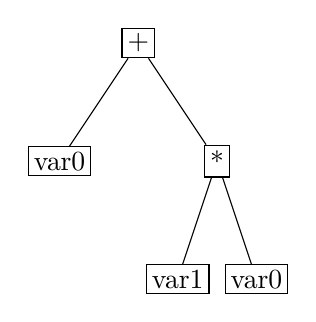
\begin{tikzpicture}
        [
        every node/.style={draw, inner sep=2pt},
        level distance=1.5cm,
        level 1/.style={sibling distance=2cm},
        level 2/.style={sibling distance=1cm}
        ]
        
        \node {+}
        child {
            node {var0}
        }
        child {
            node {*}
            child {
            node {var1}
            }
            child {
            node {var0}
            }
        };
    \end{tikzpicture}
    \caption{An example of an abstract syntax tree (AST) using deBruijn indexing. This translates to the function \texttt{f = var0 + var1 * var0}.}
    \label{fig:AST}
\end{figure}




Here, an initial DSL along with suitable syntactic constraints compile into a context-free grammar (CFG), which defines the possible structures of programs within its DSL. A CFG consists of a set of production rules that describe how to generate strings from a set of non-terminal and terminal symbols. It's "context-free" because the production rules are applied regardless of the surrounding symbols.
In DeepSynth, a prediction model is used to predict weights for a probabilistic CFG (PCFG), extending the CFG by associating probabilities with the production rules. This allows the grammar to not only generate the syntactic structure of a program but also to represent beliefs about the relative plausibility or frequency of different structures \footnote{See appendix \ref{app:cfg} for a formalization of CFGs and PCFGs.}. This is similar to DreamCoder's transition matrix which is outputted by the recognition model. The PCFG guides the search and inference process towards more likely programs. DreamCoder however, does not specifically use a PCFG. Both frameworks employ a typed $\lambda$-calculus, hence there are restrictions on program arguments, etc. (syntactical constraints). DreamCoder performs type inference during program generation. To spare computational cost, DeepSynth constructs the CFG beforehand which in turn increases the size of the CFG.

\subsubsection{\green{GFlowNet}}\label{sec:gflownet}
In the following I will give a detailed explanation of GFlowNet
\todo[inline]{should this be here or in intro? Explain why we explain this. 1. to show how the algorithm works, 2. to show how we deal with the marginalization term}

GFlowNets create a directed acyclic graph (DAG) over the state space, where vertices correspond to states or partial samples and edges denote transitions or adding a component to a partial sample, in which the edges carry a flow from source to targets \cite{bengio2023gflownet, bengio_flow_2021}.
\todo[inline]{show diagram of DAG and talk about the causality requirement! (In the methods section we explain what we do and why we do it.)}
In GFlowNets, the "flow" in the network corresponds to the process by which the network constructs a sample, which can be thought of as a path in a graph where nodes are partial samples, and edges correspond to adding a component to the partial sample.
The core training objective for a GFlowNet is to satisfy the flow matching constraint. The idea is to ensure that the flow into any state (a partially constructed sample) should match the flow out of it, given the reward associated with complete samples. The flow here refers to the expected transitions into or out of a state under the model's stochastic policy. 
Formally, a state \( s \) represents a partial object a certain stage in the generative process. A trajectory \( \tau \) is a sequence of states \( s_0, s_1, ..., s_T \) that the model traverses from an initial state \( s_0 \) to a terminal state \( s_T \), where the target structure is complete.
A trajectory \( \tau \) is formed by a sequence of actions \( a_1, a_2, ..., a_T \), where each action \( a_t \) transitions the model from state \( s_{t-1} \) to state \( s_t \). The sequence of actions is governed by a policy \( \pi \), which defines the probability of choosing a particular action given the current state.
The flow \( F(\tau) \) of a trajectory \( \tau \) is defined as the product of the probabilities of each transition along the trajectory, multiplied by the reward \( R(s_T) \) of the terminal state, normalized by a partition function \( Z \).

\begin{equation} \label{eq:flow}
    F(\tau) = \frac{R(s_T)}{Z} \prod_{t=0}^{T-1} \pi_\theta(s_{t+1} | s_{t})
\end{equation}

The partition function \( Z \) ensures that the sum of flows over all possible trajectories equals one, effectively normalizing the distribution. Since we don't know \( Z \), we can estimate it by parameterizing it as \( Z_{\theta} \).
The flow matching constraint enforces that for any given non-terminal state \( s \), the total flow into \( s \) must equal the total flow out of \( s \):

\begin{equation} \label{eq:flow_match}
    F(\tau) = F(\tau')
\end{equation}

where \( F(\tau') \) is the reverse trajectory.
We can utilize this property to create a suitable loss function to train the GFlowNet \cite{malkin_trajectory_2022}. Combining equations \ref{eq:flow} and \ref{eq:flow_match} gives us:

\begin{equation}
    \frac{R(s_T)}{Z_\theta} \prod_{t=0}^{T-1} \pi_\theta(s_{t+1} | s_{t}) = \frac{R(s_0)}{Z_\theta} \prod_{t=0}^{T-1} \beta_\theta(s_{t} | s_{t+1})
\end{equation}

Here \( \beta \) is the backward policy, predicting parent states. 
The initial state \(s_0\) has the total flow and no reward, we can rewrite it and get:

\begin{equation}
    Z_{\theta} \prod_{t=0}^{T-1} \pi_\theta(s_{t+1} | s_{t}) = R(s_T) \prod_{t=0}^{T-1} \beta_\theta(s_{t} | s_{t+1})
\end{equation}

We can now take the log on both sides:

\begin{equation}
    \log \left(Z_{\theta} \prod_{t=0}^{T-1} \pi_\theta(s_{t+1} | s_{t})\right) = \log \left(R(s_T) \prod_{t=0}^{T-1} \beta_\theta(s_{t} | s_{t+1})\right)
\end{equation}

This can be rearranged to:

\begin{equation}
    \log Z_\theta + \sum_{t=0}^{T-1} \log \pi_\theta(s_{t+1}|s_{t}) = \log R(s_T) + \sum_{t=0}^{T-1} \log \beta_\theta(s_{t}|s_{t+1})
\end{equation}

The trajectory balance loss is the squared difference:

\begin{equation}
    \mathcal{L}_{TB} = \left(\log Z_\theta + \sum_{i=0}^{T-1} \log \pi_\theta(s_{t+1}|s_{t}) - \log R(s_T) - \sum_{t=0}^{T-1} \log \beta_\theta(s_{t}|s_{t+1})\right)^2
\end{equation}

In order to mitigate the computational [cost], I am embedding all rules rather than primitives \todo[inline]{this is explained in a later section}, such that each rule is unique. Thus, every predicted node (rule) has exactly one parent, in other words, I am essentially linearising the tree. Therefore, $\beta$ will always be $1$ and can be disregarded from the equation.
Moreover, since we are solving tasks \( x \in X \), we have a conditional reward distribution $R(s_T|x)$, as well as a conditional forward policy $\pi_\theta(s_T|x)$ and partition function $Z_\theta(x)$.
This gives us the final loss:

\begin{equation}\label{form:TB}
     \mathcal{L}_{TB} = \left(\log Z_\theta(x) + \sum_{t=0}^{T} \log \pi_\theta(s_{t+1}|s_{t}, x) - \log R(s_T \vert x)\right)^2
\end{equation}     



% Formally, the computational model is as follows:
% input: tasks x in X, DSL, syntactic constraints, reward function, hyperparameters alpha, beta, epsilon, generative model, GFN

% output: trained generative model, trained recognition model, programs solving tasks X


% \subsubsection{\orange{Compositional Latent Variable Model}}
% Finetuning our fomalization, we can specify that our goal is to construct programs $z \in \mathcal{Z}$ where $z$ can be nested. We can therefore see it as a compositional latent variable model as described in \cite{hu_gflownet-em_2023}. 
% Given a set of observations \( X \), the marginal likelihood or evidence is:
% \begin{equation}\label{form:evidence}
% p(x) = \sum_z p_\theta (x|z) p_\theta(z)
% \end{equation}

% We can formalize the optimization challenge as finding the parameters \( \theta \) that maximize the data's log-likelihood:
% \begin{equation} %\label{form:bayes}
%     \mathcal{L} = \log \prod_{i=1}^{T} p(x_i) = \sum_{i=1}^{T} \log \sum_{z} p_\theta(x_i|z) p_\theta(z)
% \end{equation}

% \todo[inline]{is this correct? is the optimization challenge not over phi and theta and X?}

% The full algorithm is described in the pseudocode: \ref{alg:flowcoder}. 

\todo[inline]{We need to formalize the overall objective}

\subsubsection{\green{Expectation-Maximization}}
Hu et al. introduce a GFlowNet-EM which utilizes Expectation-Maximization in order to deal with the difficult problem of joint optimization \cite{hu_gflownet-em_2023} \footnote{See \url{https://github.com/GFNOrg/GFlowNet-EM/} for the accompanying code.}.
The core principle of Expectation-Maximization (EM) involves an iterative two-step process: the Expectation (E) step computes an expectation of the log-likelihood evaluated using the current estimate for the parameters, and the Maximization (M) step, computes parameters maximizing the expected log-likelihood found in the E-step. The GFlowNet version is slightly different and we separate the parameterization.
In the E-step the recognition model is optimized, i.e. the forward policy of the GFlowNet that is proportional to the posterior.
Here, empirical data as well as a trajectory is sampled and the trajectory balance loss is used to update the parameters of the forward policy $\pi_\phi(z|x)$, i.e. $\nabla_\phi \mathcal{L}_{TB}$.
In the M-step also empirical data and a trajectory is sampled but only the reward is used to update the parameters of the generative model $p_\theta(x \vert z) p_\theta(z)$.




\subsubsection{\green{Sleep}}
As sleep has been proven to be a crucial element of the models success, I am utilizing it too. 
\begin{description}
    \item[Replay] In Replay, I am training the forward policy on previously correctly solved task-program pairs $(x, z)$, using the trajectory to guide the model to the correct solution and optimizing on the forward logits. Here $x$ is sampled from the empirical distribution and $z$ is sampled from the forward policy $\pi_\phi$. Additionally, I apply a sleep weight $\gamma$ to strengthen the gradient. Formally:
    \begin{equation}
        \nabla_\phi\mathcal{L}_{\text{Replay}} = \mathbb{E}_{x \sim X, z \sim \pi_\phi(z|x)} \left[ - \gamma \cdot \log \pi_\phi(\tau \vert x, z) \right]
    \end{equation}
    If a correct solution has been found during the E-step, I immediately let the model train on these trajectories of correct solutions so as to consolidate these.
After the E-step I again train the model on a set (in the mathematical sense, meaning no duplicates) of all the correct solutions, so that it doesn't forget solutions to other tasks.
Replay is applied stochastically, given the hyperparameter \texttt{replay\_prob}.
    
    \item[Fantasy] During Fantasy I train the model on programs constructed during the E-step and run tasks from the empirical distribution through those programs to create correct task-program pairs $(x, z)$. Then, similarly to the methodology of Replay, I train the model on these pairs. Formally:

    \begin{equation}
        \nabla_\phi\mathcal{L}_{\text{Fantasy}} = \mathbb{E}_{x \sim X, z \sim \pi_\phi(z|x)} \left[ - \gamma \cdot \log \pi_\phi(\tau \vert x, z) \right]
    \end{equation}
    Fantasy is also applied stochastically, given the hyperparameter \texttt{fantasy\_prob}. 
    \todo[inline]{filtering out programs that produce None, constants, etc. }
    Fantasy on incorrectly proposed programs or randomly generated programs from the generative model lets the model learn which task-program pairs make sense, while fantasy on correct programs lets the model generalize solutions to different input-output pairs.
\end{description}


\subsubsection{\green{Optimization Techniques}}\label{sec:optim}
Hu et al. propose a few optimization techniques which proved to be useful \cite{hu_gflownet-em_2023}. I adapted these techniques and will describe them in the following.
\begin{description}
    \item[E-step Loss Thresholding] Rather than training the GFlowNet to a loss of zero after each M-step, we can apply a linearly decreasing moving average loss $\delta$ as a threshold to trigger the M-step using the hyperparameter $\alpha$, to save computational cost. Here I use the recursive formula:

    \begin{equation}\label{eq:threshold}
        \delta = \alpha \cdot \mathcal{L}_{TB} + (1 - \alpha) \cdot \delta
    \end{equation}
    \item[Exploration] Since we want to find many modes in the E-step and want to avoid getting stuck in local optima, several exploration techniques can be employed.
    The hyperparameter $\{\beta \vert \beta \in \mathbb{R}_{[0, 1]} \}$  can be used to exponentiate the forward policy: $ \pi_\theta(s_{t+1}|s_t)^\beta $.
    Moreover, $\epsilon$-uniform sampling can be used to the deter the model from repeating known routes by mixing the predicted logits with a uniform distribution. $\epsilon$ is chosen to be $\{\epsilon \vert \epsilon \in \mathbb{R}_{[0, 1]} \}$.
\end{description}


\begin{algorithm}[H]
    \caption{FlowCoder}
    \begin{algorithmic}[1]
    \Require Data $X$, generative model with parameters $\theta$, forward policy with parameters $\phi$, optimization and exploration hyperparameters, threshold $\alpha$
    \Repeat
        \State Sample $x \sim X$
        \State Sample $z \sim \pi_\phi(z|x)$
        \State \textbf{E-step}: gradient update on $\phi$ with $\nabla_\phi \mathcal{L}_{TB}$
        \If{$r \in (0, 1) < \texttt{replay\_prob}$}
            \State gradient update on $\phi$ with $\nabla_\phi\mathcal{L}_{\text{Replay}}$
        \EndIf
        \If{$r \in (0, 1) < \texttt{fantasy\_prob}$}
            \State gradient update on $\phi$ with $\nabla_\phi\mathcal{L}_{\text{Fantasy}}$
        \EndIf
        \If{$\mathcal{L} < \alpha$}
            \State Sample $z \sim \pi_\phi(z|x)$
            \State \textbf{M-step}: gradient update on $\theta$ with $\nabla_\theta[-\log p_\theta(x|z)p_\theta(z)]$
        \EndIf
    \Until{some convergence condition}
    \end{algorithmic}
    \label{alg:flowcoder}
    \end{algorithm}
\todo[inline]{explain algorithm, check for additional hyperparameters, etc. should the gradient update of mstep be just the reward? }






\subsection{\green{Model Architecture}}




\begin{figure*}[htbp]
    \centering
    \begin{adjustbox}{width=\textwidth}
        \begin{tikzpicture}[
            node distance=2cm, 
            auto, 
            thick,
            box/.style={
                rectangle,
                rounded corners,
                draw=black, 
                align=center,
                drop shadow,
                minimum height=1cm,
                minimum width=2cm
            },
            arrow/.style={
                ->,
                -{Stealth[length=10pt]}
            }
        ]
        
            % Nodes
            \node[box, fill=yellow!50] (task) {Task};
            \node[box, fill=yellow!70, right=3cm of task] (ioencoder) {IOEncoder};
            \node[box, fill=blue!20, below=1cm of task] (state) {State};
            \node[box, fill=blue!50, right=3cm of state] (ruleencoder) {RuleEncoder};
            
            % Positioning the Transformer node in between IOEncoder and RuleEncoder
            \coordinate (middle) at ($(ioencoder.east)!0.5!(ruleencoder.east)$);
            \node[box, fill=green!20, right=3cm of middle] (transformer) {Transformer};
            
            % Nodes for FORWARD and Z at 45 degree angles
            \node[box, fill=purple!30, above right=0.5cm and 2cm of transformer] (forward) {FORWARD};
            \node[box, fill=purple!50, below right=0.5cm and 2cm of transformer] (z) {Z};
        
            % Edges
            \draw[arrow] (task) -- (ioencoder);
            \draw[arrow] (state) -- (ruleencoder);
            \draw[arrow] (ioencoder) -- (transformer);
            \draw[arrow] (ruleencoder) -- (transformer);
            \draw[arrow] (transformer) -- (forward);
            \draw[arrow] (transformer) -- (z);
        
        \end{tikzpicture}
    \end{adjustbox}
    \caption{Insert explanation + maybe change task to an actual task; same with state; maybe also show the forward and Z output better.}
    \label{ref:model_diagram}
\end{figure*}
\todo[inline]{this looks like its one model show that the transformer output is a state representation. the GFlowNet 
 and Z takes it and produces logits.}





\begin{figure}[H]
    \centering
    % Tree 1
    \begin{subfigure}[t]{0.18\textwidth}
        \centering
        \raisebox{1.5cm}{ % Adjust vertical position
        
\begin{tikzpicture}[every node/.style={draw, circle, inner sep=2pt}]
            \node {+};
        \end{tikzpicture}
        }
        \caption{Step 1}
    \end{subfigure}
    \hspace{0.5cm} % Space between trees
    % Tree 2
    \begin{subfigure}[t]{0.18\textwidth}
        \centering
        \raisebox{0.75cm}{ % Adjust vertical position
        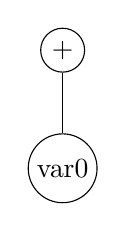
\begin{tikzpicture}[every node/.style={draw, circle, inner sep=2pt}]
            \node {+}
            child { node {var0} };
        \end{tikzpicture}
        }
        \caption{Step 2}
    \end{subfigure}
    \hspace{0.5cm} % Space between trees
    % Tree 3
    \begin{subfigure}[t]{0.18\textwidth}
        \centering
        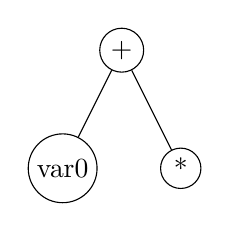
\begin{tikzpicture}[every node/.style={draw, circle, inner sep=2pt}]
            \node {+}
            child { node {var0} }
            child { node {*} };
        \end{tikzpicture}
        \caption{Step 3}
    \end{subfigure}
    \hspace{0.5cm} % Space between trees
    % Tree 4
    \begin{subfigure}[t]{0.18\textwidth}
        \centering
        \raisebox{-0.75cm}{ % Adjust vertical position
        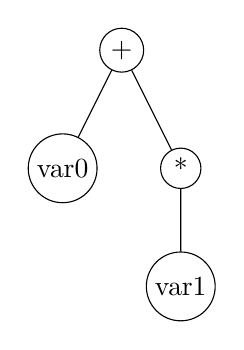
\begin{tikzpicture}[every node/.style={draw, circle, inner sep=2pt}]
            \node {+}
            child { node {var0} }
            child { node {*}
                child { node {var1} }
            };
        \end{tikzpicture}
        }
        \caption{Step 4}
    \end{subfigure}
    \hspace{0.5cm} % Space between trees
    % Tree 5
    \begin{subfigure}[t]{0.18\textwidth}
        \centering
        \raisebox{-1.5cm}{ % Adjust vertical position
        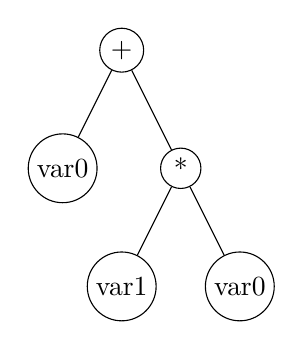
\begin{tikzpicture}[every node/.style={draw, circle, inner sep=2pt}]
            \node {+}
            child { node {var0} }
            child { node {*}
                child { node {var1} }
                child { node {var0} }
            };
        \end{tikzpicture}
        }
        \caption{Step 5}
    \end{subfigure}
    \caption{Incremental construction of the abstract syntax tree (AST) for \texttt{var0 + var1 * var0}.}
    \label{fig:AST}
\end{figure}



\begin{figure}
    \centering
    
    % Define styles for the nodes and the level distances
    \tikzset{
        every node/.style={draw, circle, inner sep=2pt},
        level distance=12mm,
        level 1/.style={sibling distance=24mm},
        level 2/.style={sibling distance=12mm},
    }
    
    % Tree at time t = 1
    \begin{subfigure}[b]{0.2\textwidth}
        \centering
        \begin{tikzpicture}
            \node {+}
                child {edge from parent[draw=none]}
                child {edge from parent[draw=none]};
        \end{tikzpicture}
        \caption*{$t = 1$}
    \end{subfigure}
    \hspace{1em} % Space between trees
    % Tree at time t = 2
    \begin{subfigure}[b]{0.2\textwidth}
        \centering
        \begin{tikzpicture}
            \node {+}
                child {node {pow}}
                child {edge from parent[draw=none]};
        \end{tikzpicture}
        \caption*{$t = 2$}
    \end{subfigure}
    \hspace{1em} % Space between trees
    % Tree at time t = 3
    \begin{subfigure}[b]{0.2\textwidth}
        \centering
        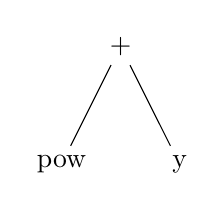
\begin{tikzpicture}
            \node {+}
                child {node {pow}}
                child {node {y}};
        \end{tikzpicture}
        \caption*{$t = 3$}
    \end{subfigure}
    \hspace{1em} % Space between trees
    % Tree at time t = 4
    \begin{subfigure}[b]{0.2\textwidth}
        \centering
        \begin{tikzpicture}
            \node {+}
                child {node {pow}
                    child {node {y}}
                    child {edge from parent[draw=none]}
                }
                child {edge from parent[draw=none]};
        \end{tikzpicture}
        \caption*{$t = 4$}
    \end{subfigure}
    
    % Tree at time t = 5
    \begin{subfigure}[b]{0.2\textwidth}
        \centering
        \begin{tikzpicture}
            \node {+}
                child {node {pow}
                    child {node {y}}
                    child {node {x}}
                }
                child {edge from parent[draw=none]};
        \end{tikzpicture}
        \caption*{$t = 5$}
    \end{subfigure}
    
    \caption{Creation of a five node tree using the grow initialization method with a maximum depth of 2, using terminal set $T$ and function set $F$ defined earlier, ($t = $ time).}
    \label{fig:growth_trees}
    \end{figure}
    


% All modules are written using PyTorch \cite{NEURIPS2019_9015}.
See table \ref{table:params} for the exact parameterization of the model.


\subsubsection{\green{Generative Model}}
To embed programs effectively within a neural network, it is essential to represent them in a format that is compatible with the neural network's architecture. Abstract syntax trees, which are inherently 2-dimensional and include information of parent, children and sibling nodes, should be translated into a neural network format while ensuring the preservation of this valuable structural information.
Various concepts have emerged, including using Graph Neural Networks (GNNs), e.g. see \cite{allamanis2017learning, velickovic_clrs_2022, Bieber_Sutton_Larochelle_Tarlow_2020, ibarz2022generalist}. Others proposed special Tree-Transformers which are able to encode ASTs, see e.g. \cite{peng_rethinking_2022, Wang_Lee_Chen_2019}.
He et al. find that standard Transformers achieve similar results to Transformers where tree position information is explicitly encoded \cite{he_trees_2021}. This is presumably because of the positional encoding, which is a way of adding fixed sinusoidal functions with different frequencies and phases to the embeddings of tokens in a sequence, enabling the neural network to discern the position of each tokens through these distinctive patterns; and more importantly, because of the fundamental component of the Transformer, which is the self-attention mechanism, formalized as \cite{Vaswani_Shazeer_Parmar_Uszkoreit_Jones_Gomez_Kaiser_Polosukhin_2017}:
\begin{equation}
    \text{Attention}(Q, K, V) = \text{softmax}(\frac{QK^T}{\sqrt{d_k}})V
\end{equation}

This mechanism, through the query (Q), key (K), and value (V) matrices, allows the model to dynamically assign importance to different parts of the input sequence. The scaling factor $\sqrt{d_k}$ normalizes the dot product, aiding in stabilizing gradients during training. Moreover, the Transformer employs Multi-Head Attention, enabling the model to concurrently process information from different representation subspaces, enhancing its capability to capture diverse features. 
Therefore, I decided to use the standard Transformer architecture, which takes a 1-dimensional sequence as an input, meaning the AST has to be linearized. 

Rather than embedding the primitives of the DSL to construct ASTs, I embed the already preprocessed rules of the context-free grammar, created in conjunction with the syntactic constraints, thus essentially predicting edges rather than nodes. The array of CFG rules has to be converted back to AST format for evaluation, which can be easily done within the DeepSynth framework.
In a plausible model of cognition, we don't possess an explicit representation of the CFG but rather infer it.
However, in the case of DeepSynth, it generates a more extensive CFG instead of conducting type inference, which is the approach employed in DreamCoder. Consequently, I must perform a lookup to identify the syntactically permitted rules, thereby filtering out those that do not conform to the syntax. Naturally, in principle, I could allow the model to generate syntactically incorrect programs and assign them a reward of 0 during evaluation, but to expedite the learning process, I refrain from doing so.

\begin{description}
    \item[The RuleEncoder] begins by collecting rules, which are pairs of non-terminals and corresponding program actions, from the CFG and adds special tokens such as 'PAD' (padding), 'START' (sequence start), and 'STOP' (sequence end). Each rule is passed through a PyTorch embedding layer.
    During the forward pass, batches of state sequences (each state sequence, or trajectory $\tau$, representing a series of CFG rules) are processed. To ensure uniformity across different sequences within a batch, padding is applied.
    \item[The IOEncoder] is tasked with encoding input-output (IO) pairs into continuous vector representations.
    Each input-output pair is tokenized using a predefined lexicon (a list of symbols representing the possible range of inputs and outputs), which includes special tokens such as 'PAD' (padding), 'IN' (input start), and 'OUT' (output start). This tokenization is critical for distinguishing between different parts of the input-output pairs.
    The tokenized input-output pairs are concatenated into a single sequence, with the 'IN' and 'OUT' tokens demarcating the transition from input to output. Padding is then applied to ensure that all sequences have the same length, aligning them to the maximum allowed size determined by \texttt{n\_examples\_max} (the maximum number of input examples that can be processed) and \texttt{size\_max} (the maximum size of elements in a list). These parameters have been adapted from DeepSynth. The padded sequences are passed through a PyTorch embedding layer. This embedding is crucial for capturing the semantic relationships between different tokens.
    \item[The Transformer] initializes with the IOEncoder and the RuleEncoder. Positional Encoding is applied to the output of both encoders. This step is vital as it adds information about the sequence order to the model, allowing the Transformer to interpret the sequence data effectively.
    The Transformer employs two types of masks: padding masks for IO sequences and square subsequent masks for state sequences. The padding mask ensures that the model does not process padding tokens, while the square subsequent mask prevents positions from attending to subsequent positions, maintaining the autoregressive property in the generation process.
\end{description}

\subsubsection{\green{Forward Policy}}
At each step, the forward policy takes the Transformer output as an encoded state and predicts log probabilities over the CFG rules, after which I apply softmax to get a distribution between 0 and 1 and sample the next action. 
The forward policy is implemented as a Multi-Layer Perceptron (MLP) and predicts forward logits from the Transformer's output, guiding the generative process.

\subsubsection{\green{Partition Function}}
The partition function $Z_\theta$ serves as a normalizing factor, ensuring that the probabilities generated by the model are well-calibrated and interpretable. It is implemented as a MLP layered on top of the Transformer output.

\subsubsection{\green{Sampling Programs}}
In the process of constructing an Abstract Syntax Tree, there exists flexibility in the order of expansion. Nodes can be expanded in a depth-first, breadth-first, etc. manner, or for instance, one can adopt a bottom-up approach, wherein terminal nodes are predicted initially and subsequently connected in a progressive manner. This approach offers the advantage of enabling the evaluation of partial expressions, which, in turn, can serve to inform the model and enhance computational efficiency, albeit at the expense of increased memory requirements. Alternatively, we may consider employing a model akin to the forward policy, predicting the subsequent node (or edge) to be expanded.
However, I chose to sample the actions for the tree construction in a depth-first manner. I did this for two reasons. 
First, for simplicity, to not overcomplicate the model, and second so that the AST when linearized, always has the same order, potentially giving the Transformer a useful inductive bias.

Specifically, the state of each program in the batch is initialized with a 'START' token, representing the initial state of the program generation process. A frontier, implemented as a queue, is initialized for each program to manage the sequence of non-terminals that need to be expanded. This method has been adapted from DeepSynth to fit with the FlowCoder framework and mechanisms. 
The core of the method is a loop that continues until all frontiers are empty, indicating that all programs in the batch have been fully generated. Within this loop, the model computes logits and partition functions.
As discussed in section \ref{sec:optim}, the sampling method includes an exploration mechanism, where with a probability $\epsilon$, uniform sampling is used instead of the model's logits. This exploration is crucial for introducing variability and avoiding local optima in the generation process. Additionally, tempering is applied to logits using a factor $\beta$, modulating the sharpness of the probability distribution used for sampling.
For each program in the batch, the method iteratively samples a rule based on the current non-terminal and updates the program's state and cumulative logits. This process involves creating a mask to block invalid actions, applying the mask to logits, and sampling an action (rule) based on the masked logits.
Each sampled rule is decomposed into a non-terminal and program component, updating the program's current state and expanding the frontier with the rule's arguments.
Once all frontiers are empty, the final programs are reconstructed from their compressed representations, using methods provided by DeepSynth.

\todo[inline]{Refer to program construction diagram}
\todo[inline]{detailed algorithm of replay and fantasy}

\subsubsection{\green{Reward}}
In order to train the model, we need to operationalize a reward function. Various approaches exist for this purpose, the simplest being a binary reward, as employed in DreamCoder. Does the output of the program match the actual output or not? A binary reward however, is not very informative. A reward that provides a gradient is much more useful. Bengio et al. propose an Energy-Based Model (EBM), wherein the model learns to associate favorable outcomes with low energy states and unfavorable outcomes with high energy states \cite{bengio2023gflownet}. Depending on the domain, this may be useful but in my experiments, working in the list editing domain, however, I found that it introduced unnecessary complexity to the model. Instead, I am using the Levenshtein edit distance, using the \texttt{Levenshtein} package \footnote{\url{https://github.com/maxbachmann/Levenshtein}}, which is a measure of the similarity between two strings. Specifically, it quantifies the minimum number of single-character edits (i.e., insertions, deletions, or substitutions) required to transform one string into another. See appendix \ref{app:levenshtein} for an in depth formalization of the metric.
Since the Levenshtein distance returns a discrete value, I normalize it over the maximum length of the sequences, and since there may be more than one example per task, I average it over all examples. Moreover, I apply a maximum reward parameter, to scale a correct solution up and give the model a stronger gradient. In my experiments I used a maximum reward of 10.















\subsection{\green{Design}}
In the following section I will elaborate on the exact training and test methods I used, including hyperparameters.
The tasks I am using are input-output relations in the list editing domain, originally from DreamCoder, see Table \ref{tab:task_ex} for examples. These were filtered given the syntactic constraints (e.g. type, lexicon, etc.) and provided by DeepSynth. 
In their paper, Fijalkow et al. discuss that some of the tasks are impossible solve given the DSL, so I additionally filtered those out. In my experiments I end up with 95 tasks. Tasks can be of a similar variety (e.g. \texttt{add-k with k=1} and \texttt{add-k with k=2} belong to the same group). There are 25 such task groups in total. Each task can have between 1 and 15 examples. A task is considered solved if a program solves all examples of the task \footnote{All tasks can be found in my GitHub repository.}.
The DSL is essentially a dictionary of primitive types and semantics in a typed $\lambda$-calculus, including functions like \texttt{index}, \texttt{car}, \texttt{append} as well as numerical functions like \texttt{+}, \texttt{*}, \texttt{mod}, \texttt{is-prime}, etc., all written in Python (see appendix \ref{app:dsl}).
Table \ref{tab:synconst} describes the syntactical constraints used in the experiment, which were mostly adapted from DeepSynth and DreamCoder.

\begin{table}[H]
    \centering
    \begin{tabularx}{\textwidth}{|l|l|X|}
        \hline
        \textbf{Parameter} & \textbf{Value} & \textbf{Description} \\\hline
        \texttt{type} & \texttt{list(int) $\rightarrow$ list(int)} & The input as well as the output should be a list of integers, so the CFG should reflect that, filtering rules that do not conform to that criterion. \\\hline
        \texttt{lexicon} &  $[-30, 30] \in \mathbb{Z}$ & The lexicon is a uniform distribution of integers and in the range from -30 to 30 \\\hline
        \texttt{maximum argument number} & 1 & This is the maximum number of arguments a function could have. \\\hline
        \texttt{size max} & 10 & The maximum number of values in a list \\\hline 
        \texttt{max number of examples} & 15 & The maximum number of examples per task \\\hline 
    \end{tabularx}
    \caption{Syntactical Constraints}
    \label{tab:synconst}
\end{table}

All experiments were trained in random order with a batch size of 4 where each task in the batch is the same. This was done to avoid a credit assignment problem while increasing efficiency. Since the forward logits are summed up and averaged over for all trajectories, training the model at multiple task at once might have confused which trajectory was rewarding. However, batching, especially when training on a GPU has computational benefits.
Furthermore, each task is trained for 5 epochs with 2.000 E-steps and 2.000 M-steps in each epoch. The moving average threshold (see equation (\ref{eq:threshold})) $\delta$ was initialized with 150 and linearly decreases using the hyperparameter $\alpha$ set to 0.3. The exploration parameters $\beta$ and $\epsilon$ were set to $0.7$ and $0.3$, respectively. The sleep weight $\gamma$ was set to 10 on all experiments. 
The learning rates for the generative model as well as for the forward policy were set to $0.0001$. During inference I ran the model for $100$ steps. Since the batch size is 4, this creates 400 programs per task. A table of all hyperparameters can be found in Table \ref{tab:hyperparams} of appendix \ref{app:hyperparams}. The experiments were run on a single NVIDIA Tesla T4 GPU. Throughout the five epochs, each consisting of 2.000 E- and M-steps with a batch size of four, the model generated approximately 80.000 programs per task.

\begin{table}[H]
    \centering
    \begin{tabular}{|p{5cm}|c|c|}
        \hline
        \textbf{Task} & \textbf{Input} & \textbf{Output} \\\hline
        \texttt{remove gt 2} & \texttt{[1,2,7,5,1]} & \texttt{[1,2,1]} \\\hline
        \texttt{caesar-cipher-k-modulo-n with k=5 and n=4} & \texttt{[2, 2, 0, 1, 2, 3, 3]} & \texttt{[3, 3, 1, 2, 3, 0, 0]} \\\hline
        \texttt{prepend-index-k with k=3} & \texttt{[15, 12, 9, 14, 7, 9]} & \texttt{[9, 15, 12, 9, 14, 7, 9]} \\\hline
        \texttt{add-k with k=4} & \texttt{[16, 10, 7, 12, 13, 3]} & \texttt{[20, 14, 11, 16, 17, 7]} \\\hline
        \texttt{append-k with k=2} & \texttt{[1, 5, 15]} & \texttt{[1, 5, 15, 2]} \\\hline
    \end{tabular}
    \caption{Task Examples}
    \label{tab:task_ex}
\end{table}



\begin{table}[H]
    \centering
    \begin{tabular}{|p{5cm}|c|}
        \hline
        \textbf{Task} & \textbf{Program} \\\hline
        \texttt{remove gt 2} & \texttt{(filter (gt? 3) var0)} \\\hline
        \texttt{caesar-cipher-k-modulo-n with k=5 and n=4} & \texttt{(map (mod 4) (map (+ 5) var0))} \\\hline
        \texttt{prepend-index-k with k=3} & \texttt{(cons (index 2 var0) var0)} \\\hline
        \texttt{add-k with k=4} & \texttt{(map (+ 4) var0)} \\\hline
        \texttt{append-k with k=2} & \texttt{(append 2 var0)} \\\hline
    \end{tabular}
    \caption{Examples of tasks and programs solving the tasks.}
    \label{tab:task_programs}
\end{table}

\newpage

\section{\green{Results}}\label{sec:results}

\subsection{\green{Experiment 1}}\label{exp:1}
This experiment tested the model's ability to generalize to unseen tasks. I set the program depth to 4 and trained on a random selection of only 17 out of 95 tasks. I set both the \texttt{replay\_prob} as well as the \texttt{fantasy\_prob} parameters to 1, increasing the sleep frequency.
Replay and fantasy are applied within each E-step, whenever a correct solution is found as well as after each E-step.
All correct task-program pairs are saved and trained on after each E-step. The training took approximately one week. The model solved 15 tasks during training and 33 during inference. Notably, 8 tasks solved in training were not solved during inference, suggesting the model occasionally lost correct solutions found during training. During inference, the model therefore solved 26 tasks it had not seen before. Out of these, 7 were from previously unobserved task groups, demonstrating the model's capacity for generalization.

\subsection{\green{Experiment 2}}
In this experiment I want to examine the model's frequency of resampling, whether the model proposes varied solutions, and analyse its efficiency. Moreover, I analyze whether the EM cycles prove to be useful.

In this experiment I trained the model on a random 50/50 train-test split, which took about 3 days. All programs can be solved with a maximum program depth of 3, so I limited the model to that depth. This was merely done for efficiency. Moreover, \texttt{replay\_prob} and \texttt{fantasy\_prob} were set to 0.3 and 1, respectively, and only a set (meaning no duplicates) of correct task-program pairs were saved and trained on, limiting the model's exposure to already correctly solved tasks [see sec for discussion on sleep]. 
The model successfully solved 33 out of the 48 tasks it was trained on. Although the model was trained on half of the tasks in the dataset, it does not generalize as well as FlowCoder in the first experiment. Sleep seems to be a crucial aspect of the algorithm.

As depicted in Figure \ref{fig:program_variations_binary_train}, an average of about 11.000 unique programs were created per task, indicating that approximately one-eighth of the programs were resampled, while the rest were distinct. This data also reveals certain task groups that posed more significant challenges than others. For instance, none of the tasks in the \texttt{caesar-cipher-k-modulo-n} group were solved, whereas all tasks in the \texttt{prepend-index-k} or \texttt{mult-k} groups were successfully completed. Refer to Tables \ref{tab:task_ex} and \ref{tab:task_programs} for examples and correct solutions, respectively.

\begin{figure}
    \centering
    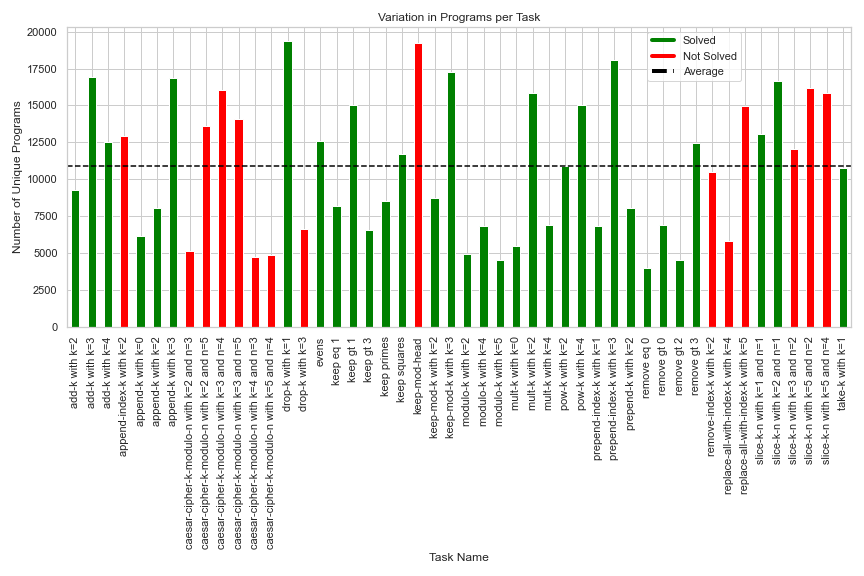
\includegraphics[width=\textwidth]{../img/plot_program_variations_binary_depth_3_48_tasks2023-12-07 22:24:45.png}
    \caption{Bar plot of unique programs created per task. The sorted tasks the model has been trained are on the x-axis and the number of unique programs that have been created per task are on the y-axis. Bars of tasks that have been solved are coloured green and unsolved tasks are coloured red. The black dotted line demarcates the average number of uniquely created programs.}
    \label{fig:program_variations_binary_train}
\end{figure}

During inference, the model attempted to solve all 95 tasks sequentially, producing 400 programs in about 100 steps, taking roughly 30 seconds for each task. FlowCoder solved 42 tasks, of which 13 were unseen during training, as shown in Figure \ref{fig:solution_variations_inference}. 11 of these tasks belong to groups where at least one task was solved during training, e.g. the model was trained on (and solved) tasks \texttt{append-k} with \texttt{k=0, k=2, k=3} and during inference the model solved tasks \texttt{append-k} with \texttt{k=1, k=4, k=5}, which were previously unseen. 2 tasks were solved during inference without any precedent of tasks of a similar task group being seen in training. Additionally, all tasks solved exclusively during inference had not been exposed to the model in the training phase.
The distribution of unique solutions also reveals that multiple tasks, irrespective of their exposure during training, exhibited a range of solutions. 
This diversity in solutions reflects the model's capacity to explore the solution space comprehensively, aligning with our goal of not merely finding a point estimate but understanding the entire posterior distribution of solutions for each task.

\begin{figure}
    \centering
    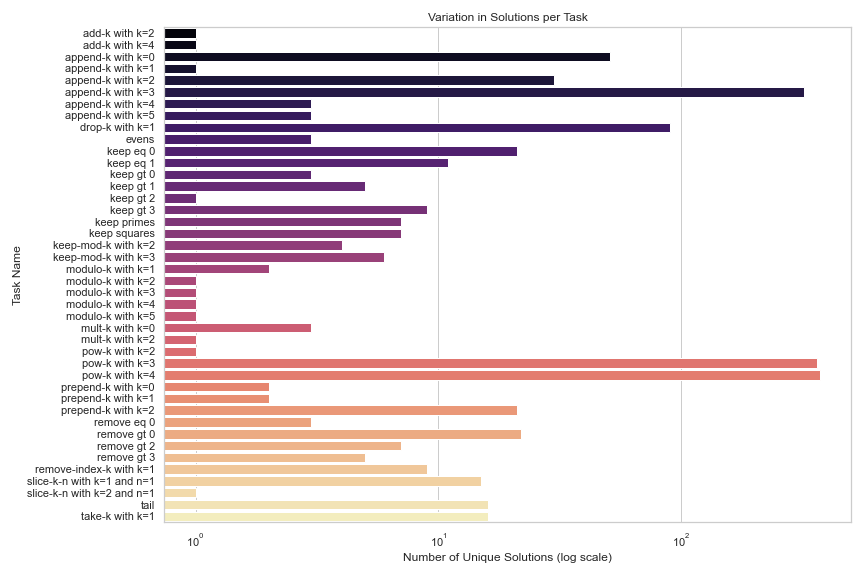
\includegraphics[width=\textwidth]{../img/plot_solution_variations_depth_3_48_tasks2023-12-07 22:24:45_inference.png}
    \caption{Distribution of unique solutions per task during inference, displayed in a log-scaled bar chart. The y-axis lists the task names, while the x-axis quantifies the number of unique solutions. The chart reveals that 13 tasks not solved in training were resolved during inference, with 11 belonging to groups with at least one task previously solved in training. Only solved tasks are shown.}
    \label{fig:solution_variations_inference}
    \end{figure}

In table \ref{tab:multiple_solutions} we can see an example of varied solutions to a task. The model has found the shortest solution but also alternate solutions of the same task.

\begin{table}
    \centering
    \begin{tabular}{|l|c|}
        \hline
        \textbf{Task} & \textbf{Solution}  \\\hline
        \texttt{append-k with k=2} & \texttt{(append 2 var0)} \\
        \texttt{} & \texttt{(append (mod 4 2) var0)} \\
        \texttt{} & \texttt{(append (min 4 2) var0)} \\
        \texttt{} & \texttt{(append (mod 5 2) var0)} \\
        \hline
    \end{tabular}
    \caption{Multiple found solutions.}
    \label{tab:multiple_solutions}
\end{table}

On average, FlowCoder efficiently solves a task within approximately 8 steps. Notably, as illustrated in Figure \ref{fig:plot_min_step_for_solution_inference}, around half of the tasks are successfully resolved on the initial attempt. The model is able to rapidly solve many tasks that it had not encountered previously, often requiring fewer steps than the average. This suggests that when trained to convergence, the model may act as an efficient sampler. 

\begin{figure}
    \centering
    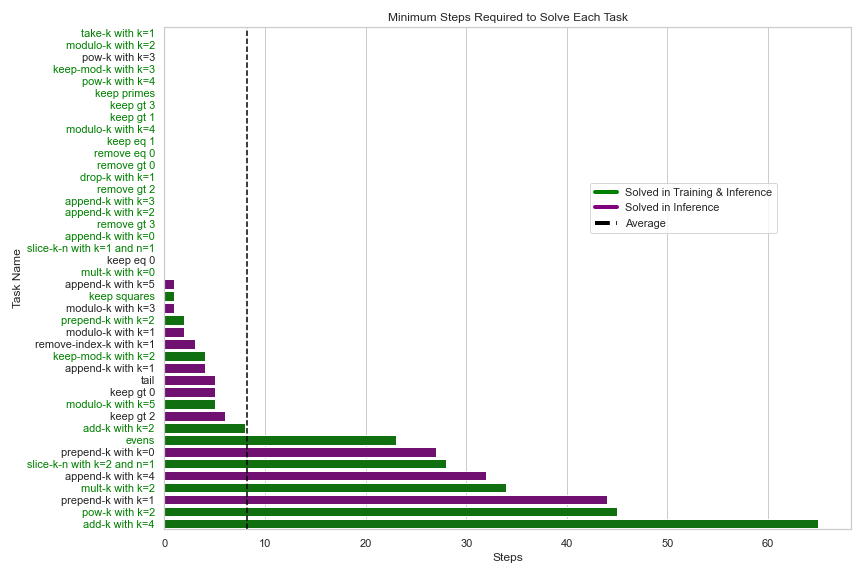
\includegraphics[width=\textwidth]{../img/plot_min_step_for_solution_inference_depth_3_48_tasks2023-12-07 22:24:45_inference.png}
    \caption{Analysis of the minimum number of steps required to solve tasks during inference. The x-axis represents the number of steps, and the y-axis lists the task names, sorted by the number of steps taken to find a solution. The dotted line indicates the average number of steps needed. Tasks solved both during training and inference are highlighted in green, whereas tasks exclusively solved during inference are in purple. Only solved tasks are shown.}
    \label{fig:plot_min_step_for_solution_inference}
\end{figure}

An examination of the model's improvement across consecutive Expectation-Maximization (E-M) cycles is shown in Figure \ref{fig:em_cycles}. The plot shows a clear upward trend in the average cumulative number of solutions, suggesting progressive improvement in both the forward policy and the generative model. The results of experiment 1 \ref{exp:1} are similar. As expected, the generative model during the M-step performs better than the GFlowNet during the E-step, since the E-step includes exploration while the M-step does not.

\begin{figure}
    \centering
    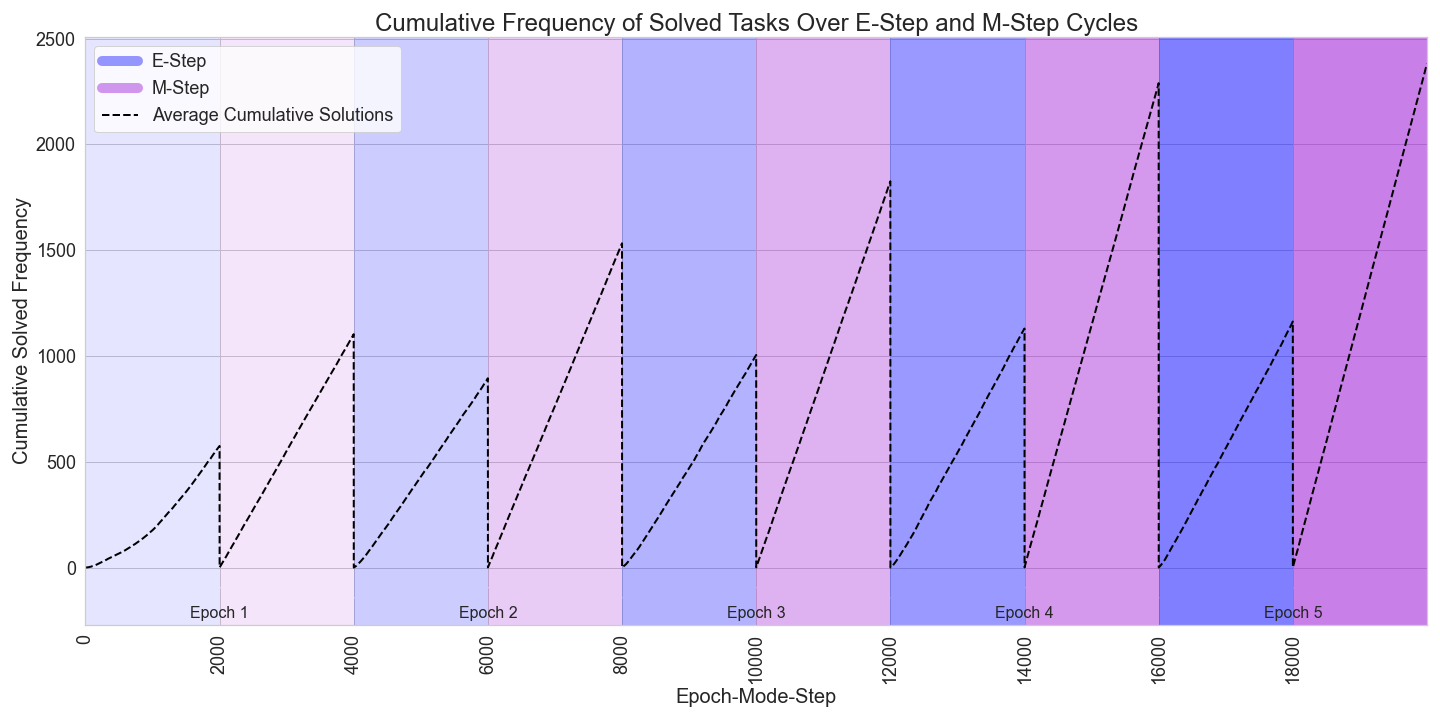
\includegraphics[width=\textwidth]{../img/em_cycles_depth_3_48_tasks2023-12-07 22:24:45.png}
    \caption{The plot displays the cumulative number of tasks solved (y-axis) against the number of steps (x-axis). Each step represents an iteration in the E-M cycle. The initial 2.000 steps correspond to the first E-step, marked with a blue background, followed by the first M-step spanning the next 2.000 steps (up to step 4.000), distinguished by a purple background. This pattern constitutes one complete epoch. The graph includes a dotted line representing the average number of tasks solved over all epochs, offering a benchmark for comparison. Furthermore, the intensity of the color hue in the plot encodes the temporal sequence of the epochs: brighter bars on the left signify earlier epochs (the first epoch), with the hue gradually darkening towards the right, culminating in the fifth and final epoch.}
    \label{fig:em_cycles}
\end{figure}


% Figure \ref{fig:program_variations_binary_inference} demonstrates the variance in task difficulty during inference. The \texttt{caesar} tasks often resulted in similar solutions, as seen from the limited diversity in program attempts, whereas a broader range of strategies was explored in other unsolved tasks. The solved tasks showed varying degrees of program exploration. On average, approximately 145 unique programs were generated per task.

% \begin{figure}[H]
%     \centering
%     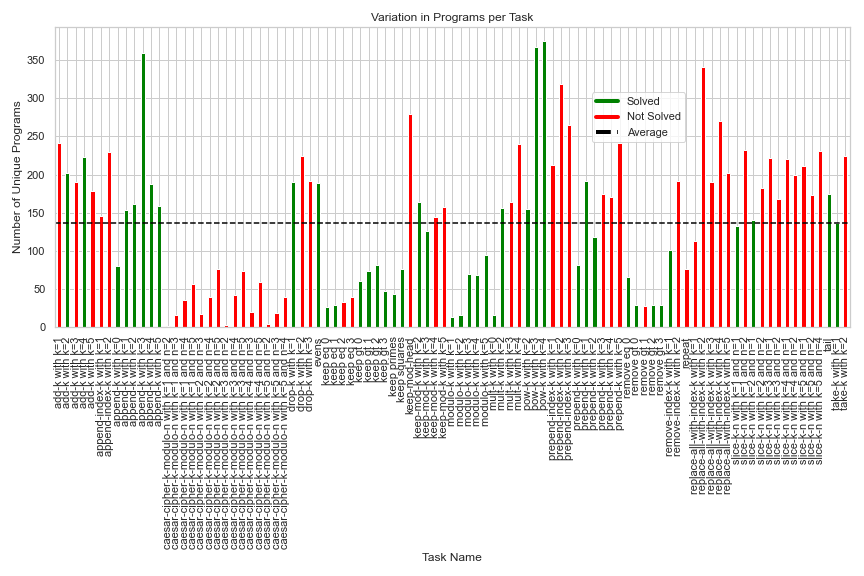
\includegraphics[width=\textwidth]{../img/plot_program_variations_binary_depth_3_48_tasks2023-12-07 22:24:45_inference.png}
%     \caption{Analysis of the number of unique programs generated per task during inference, as shown in Figure \ref{fig:program_variations_binary_inference}. Tasks are listed on the x-axis, and the count of unique programs is on the y-axis. The figure highlights the variance in program generation across tasks, with \texttt{caesar} tasks often showing limited program diversity, in contrast to other tasks that exhibit a wide range of attempts. The average number of unique programs created per task is approximately 145, indicating varied program attempts.}
%     \label{fig:program_variations_binary_inference}
% \end{figure}

% \todo[inline]{maybe take this plot out?}


\newpage
\section{\orange{Discussion}}
In this section I will summarize key findings, and address the aims of the research.


what do we want from the model?
- it should not resample too often, about an eighth (this can be improved). of course we are counting the correct solutions too, over and over 
- it should be fast (when converged, it's immediate) (however everythong above depth 4 was critical)
- it should generalize OOD (it solves previously unseen tasks within and outside of task group)
- sleep is crucial

In the following section, I will compare FlowCoder to the concepts introduced in section [introduction or more specific 1.1, 1.2, etc.]

\subsection{\orange{Experimental Results}}

\begin{itemize}
    \item since the model solves most tasks within groups, it seeps to suggest that it learns relationships between groups (program space). 
\end{itemize}

The experiments of section \ref{sec:results} revealed that FlowCoder can be trained as an adequate program synthesizer. 
First, we found that the model solves more tasks in inference than in training, including tasks of groups which had previously been unseen, suggesting some out-of-distribution generalization capabilities.
Moreover, the model produces varied solutions, not only converging on a point estimate, the most likely program, but even in inference proposes multiple programs solving the tasks, suggesting that it has found a multi-modal distribution. 
In section [x] we have discussed why a multitude of representations are useful. In the context of program synthesis however, we must not conflate semantics with syntax [see discussion]. As shown in table \ref{tab:multiple_solutions}, many inefficient alternate solutions to a task were found. We would actually like to avoid programs that add 0, multiply by 1, etc. Breaking syntactic symmetries can be done by optimising for minimum description length and including an abstraction phase as is done in DreamCoder.
The model is able to sample varied correct solutions on the first step, suggesting that when we make the investment of training the model to convergence, we reap the benefits in the form of one-shot inference.
The model's performance steadily increases with alternating E-M steps, suggesting that it is beneficial to train the generative model separately from the forward policy and having the two models bootstrap each other. The generative model proposes better representations of the program space while the forward policy selects better actions, proportional to the posterior distribution, given the task at hand.


Many tasks have not been solved, but it looks like if the model had been kept training, it could converge on those too.
moreover, we need to adjust resampling since some tasks have not been solved but have been resampled many times.


- finding a balance between 
- exploration (beta, epsilon, fantasy) to find many modes, E-step
- exploitation (replay) converging on modes, not forgetting, M-step
and exploitation (exploration to find many modes) but also exploitation





Fijalkow et al. compare different search strategies and show that methods that do not use a machine-learned PCFG (e.g. depth-first search (DFS)) barely solve any tasks (max. 5) in over 1.5 hours \cite{fijalkow_scaling_2021}. [this should be in intro]


\begin{itemize}
    \item More tasks were solved in inference. since im going chronologically through the training set, the model doesn't see the first task ever again. this would be beneficial. minibatch sampling. 
    \item there are many other training strategies that could be employed.
    \item symmetry breaking. we want to avoid if True, or $+0$ or $*1$, etc.
\end{itemize}


\begin{itemize}
    \item benefit over dreamcoder etc. we can ask questions about partial programs. we are embedding programs as well as tasks, we can input a partial program into the model and ask what the next best step is. We can also train from partial tasks etc. making this method more dynamic. [to introduction?]
\end{itemize}



\begin{description}
    \item[Sampling strategy] ASTs can be constructed in various orders. Ideally, we could let the GFlowNet predict which node to expand. However, this would have meant creating an additional model as a node predictor, which increases FlowCoder's complexity. Moreover, since ASTs are inherently two dimensional and I am using a transformer to encode CFG rules as a representation of a program, ASTs have to be linearized. I decided to expand the tree in order of depth-first, both to eliminate the need for another model and also to give the transformer the input in consistent order, making learning easier. 
    \item[] - bottom-up construction could be beneficial as nodes can already be evaluated
    - construction order
    - include diagram
\end{description}










% Similar to both approaches, I am separating the generative model from the recognition model

DreamCoder enforces parsimonious programs during abstraction. Common patterns are refactored, shortening the programs. Deepsynth enforces programs of minimum description length by optimising for the expected number of programs before finding a correct solution. This works, if programs are considered in order of increasing length. Both of these methods however optimise for point estimates, i.e. the most likely program for a given task. Instead, I want to learn the posterior distribution, i.e. all solutions to a task, which of course is much harder.
I do this, first, because if we see that the model finds the posterior, it can always be simplified to MAP. Second, given the analogy of humans understanding the world via program-like concepts, we know that we can represent the world in various ways and we can find multiple solutions to a problem. Consider the following example: the task 
% [2,,6,8] -> 
% [1,2,3] -> [2,4,9]
% Surfaces and Essences analogy example abc:xyz :: abd: (wyz/ xya) 
% [123][987]
% abc xyz
% abd wyz/ xya


I constrain the program depth to 3, which is enough to solve most programs and is not too computationally heavy.
Since most tasks can be solved by short programs, 
Despite the minimum description length being a factor which may be necessary, I relax this condition






\subsection{\orange{Comparison to DreamCoder}}


\subsection{\orange{Speed}}
It is somewhat difficult to compare the time efficiency of my method with other approaches for various reasons. 
Both DeepSynth and DreamCoder predict weights for the PCFG and then parallelize search processes on multiple CPUs. DreamCoder train their model for about a day on 20-100 CPUs and it takes around 10 wake-sleep cycles to converge in the list domain. I instead am working on one GPU (with possible interruptions from other users on the cluster). DreamCoder shows that the refactoring algorithm used in abstraction is crucial in the list processing tasks, which I did not implement.
DeepSynth does not include model query time in their computations.
I am training my model on a filtered set of the original DreamCoder dataset, making it difficult to compare with DreamCoder and some of the DeepSynth experiments. 

[Moreover, I did not work too much on time optimizations and still it seems that it isnt too slow in a rough comparison with those other methods.]









\subsection{\green{Scaling the Model}}

\todo[inline]{check this, check what is necessary}

The time complexity for encoding an IO pair is \(\mathcal{O}(n)\), where \(n\) is the length of the IO pair. 

Similarly, the RuleEncoder's time complexity is \(\mathcal{O}(n)\) where \(n\) is the number of rules.

In each step of the trajectory, I embed the task and the current state, and use the transformer to construct the trajectory until completion. 

The transformer's complexity is \(O(num\_layers \times (d_{model}^2 \times n_{seq} + n_{seq}^2 \times d_{model}))\), where \(num\_layers\) is the number of layers, \(d_{model}\) is the model dimension, and \(n_{seq}\) is the sequence length.

The linear layers within the forward policy $\pi_\theta$ and partition function $Z_\theta$ have a complexity of \(O(d_{model}^2)\) due to the matrix multiplication involved.

The overall time complexity of a forward pass through FlowCoder is dominated by the transformer's complexity, which is \(O(num\_layers \times (d_{model}^2 \times n_{seq} + n_{seq}^2 \times d_{model}))\).

Since I have linearized the construction procedure, I reconstruct the list back to AST format and then evaluate the tree to get the program output.

The reconstruction and evaluation are both recursive processes that depend on the depth of the tree and number of arguments in each partial program. 
The worst-case complexity of program reconstruction, as well as the evaluation can be approximated as \(O(k^d)\), where \(d\) is the depth of the recursion, which corresponds to the length of the program list, and \(k\) is the average number of arguments for each function in the program. In my experiments only one argument per function is allowed.

[sec x to see how we can mitigate this (better program representation, construction, evaluation (instead of reconstruction, reformating etc. ))]
In general i want to show that the model scales. 

Subsequently, I compute the reward.

The Levenshtein edit distance algorithm, when implemented using dynamic programming, has a time complexity of 
$\mathcal{O}(m \times n)$, where $m$ and  $n$ are the lengths of the two input strings.
\subsubsection{Scaling}
\begin{itemize}
    \item Scaling the model (How does the model scale with larger CFGs?)
    \item We need to show that with abstraction, we could theoretically scale
    \item Scaling neural search paper
    \item how would it work using GFNs
    \item how would it work if we use abstraction like in DC? DC shows it is scalable.
    \item this needs to be related to increasing number of primitives, maybe look at dreamcoders complexity. we save complexity by not having to search, and also space, since we dont have to save anything, we just need to train a phat model
\end{itemize}
    


The scalability of the model depends on various factors. First, we have seen that GFN can deal with the marginalization term and is an instance of amortized bayesian inference. This means that we can capitalise on seen data to generalise to many modes even in high-dimensional spaces. [show that amortized inference scales]
The intention of this study is to show that the general method of using GFNs for program synthesis is useful and not to optimise it for efficiency and scalability. Many adjustments can be made to accommodate for scaling. 
program representation, 
choosing the generative and forward (and possibly backward) policy models, 
parallelizing tasks,
different training strategies
most importantly, as discussed in [sec DreamCoder], the abstraction phase is crucial to narrow the depth of the search tree. (and MDL). 
The end-goal is to have an increasing DSL as well. 
Scaling neural search paper
all of the program construction/ reconstruction/ evaluation can be reduced. 


the problem with scaling is marginalization. DC deals with this by marginalising over a beam of programs for each task. GFN deals with it by adhering to the flow objective. 
other amortized variational inference methods, \dots






















\subsection{\orange{program representation}}
Other ideas to represent ASTs are GNNs, or Tree-Transformers [which were explored, but the computational complexity gets higher [source]. also distributed representations of aggregations are an option like in GFN-EM.], however, I settled on using a regular transformer, since it has been shown that it can learn tree structures implicitly, through positional encoding and also [source] show that the performance is similar.
since we are representing trees, it might be beneficial to embed programs in hyperbolic space [see conceptual spaces]. 
There are other ways to embed the cfg, [e.g. see kim].
- 3-index bigram, .. compound PCFG including information of neighboring states, parents, childrewn, etc. 



since we are representing the tree as an array of rules, so that we can use them with transformer, we need to reformat it back into a tree to evaluate it. i.e. we need to fisrt construct it and then go through it again for evaluation. this slows down the computation. 


- heapsearch, evaluation, using sub-trees, etc. 
Another expansion is using a depth first search (DFS) [source] approach (note that this is not about searching through the CFG, but constructing the AST). Since we are essentially linearising a tree when giving it as input to the transformer, the transformer has additional order information, which in combination with positional encoding lets it learn better. 

hyperbolic space



We could embed parent, child, etc. to make ean embedding of a rule more informed. i chose not to do it to see whether its enough (discuss in limitations,e tc. )

Syntax vs Semantics 
Semantics can be understood as data flow, e.g. partial evaluations could be used as part of the representation of the program. 
type information 
For a discussion on semantics and meaning see sec [meaning]
In LLMs, we see that they l









\subsection{\red{Program Embeddings}}
programs are commonly represented as AST. 
% Although these models are great, their method reveals a foundational limitation: their heavy reliance on syntactical constraints. While these constraints are undoubtedly vital for ensuring the correctness of generated programs, they do not necessarily guarantee a deep understanding or utilization of semantic relationships within the code. 
% A lot of information may be lost, by disregarding the semantic relationships. As we have seen in [reference LLMs], there seems to be a semantic grammar on top of the syntactical structure of the language which we may be able to leverage.
% This has been criticized in [cite all the relevant papers (using GNNs, etc. ) also Kim's neural PCFG].
% Perhaps we can utilise transformers to learn a "program space", a kind of neural probabiilistic context-free grammar

% - we could imagine a program space in which symmetries [reference] and so on could be leveraged. For example, one could argue that "\(+\)" is to "\(-\)" as "\(\div\)" is to "\(\times\)", and anyways once we create programs which really represent actual concepts, the same regularities should be systematically compressed.

Does DC learn a program space (discuss their tsne)
- hyperbolic

Graph Neural Networks seem like an interesting option to represent ASTs
Allamanis et al. use Gated Graph Neural Networks to include local semantics in their program representations 

Allamanis et al. use Gated Graph Neural Networks to represent both syntactic and semantic information by including data flow and type hierarchy signals \cite{allamanis2017learning}. The authors formalize how to turn ASTs to graphs.

Wang et al. propose a semantic program embedding, learnt from program execution traces \cite{wang2017dynamic}.

Ibarz et al. present a generalist neural algorithmic learner by leveraging GNNs \cite{ibarz2022generalist}.
Zhang et al. propose a novel neural AST representation of source code \cite{zhang_novel_2019}.

Oliviera and Löh develop abstract syntax graphs (rather than trees) to preserve sharing and recursion within a DSL \cite{oliveira_abstract_2013}.









\subsection{\red{reward}}

\begin{itemize}
    \item Reward should be learnt (Energy based model). Where does the brain get it from?
    \item Is Levenshtein a reasonable reward? think about computational complexity (Kolmogorov complexity)
    \item Reward depends on tasks
    \item Rewards can be based on utility or efficiency rather than accuracy, or on aesthetics or other determinants. This is a complex topic which should be investigated in the future. 
\end{itemize}






\subsection{\red{Limitations}}
\begin{itemize}
    \item Make the network choose where to expand (not DFS). Note that we are not going through the CFG DFS, but creating the AST with DFS (GNN, evaluation etc. )
    \item What should be the best order of solving tasks? should we try to solve a certain task for x amount of time and then move on to the next? curriculum learning? 
    \item Better reward
\end{itemize}









\subsection{\red{Related Work}}
\begin{itemize}
    \item apperception engine
    \item one language to rule them all
    \item 
\end{itemize}

\subsection{\red{Future Work}}
\begin{itemize}
    \item testing sleep, exploration, etc. 
    \item Sub-trajectory balance
    \item Learning from dataset of good programs (akin to someone telling you a solution)? 
    \item Train from middle of states
    \item Train backward policy, then we can also see finished states and predict trajectories that led to them
    \item caching evaluations, bottom-up
    \item we could let automate how long to train. if it is solving the task in 100 consecutive e steps and also in m stepts, it could also just move on. 
    \item Hyberbolic space (relate to holarchies)
\end{itemize}
































\subsubsection{\orange{Comparison to other approaches}}

Previously, techniques in approximate Bayesian inference, have been applied to deal with the difficult marginalization term.

Variational Inference (VI) is a strategy that leverages a simpler distribution \( q(z | x) \)  to approximate a more complex target distribution. This is achieved by minimizing the Kullback-Leibler (KL) divergence, a similarity measure of probability distributions, between the true distribution and its approximation.

\[
    D_{KL}[q(z|x) || p(z|x)]
\]

The approximation can be optimized by increasing the Evidence Lower Bound (ELBO) by:

\begin{equation}
\text{ELBO} = E_{q(z|x)}[\log p(x|z)] - D_{KL}(q(z|x) || p(z|x))
\end{equation}
Where \( E_{q(z|x)} \) denotes the expectation under the recognition density \( q \).

In the context of \emph{amortized} VI, computation of the variational parameters \( \phi \) is shared across multiple data points. Traditional VI might determine a unique set of variational parameters \( \phi_i \) for each data point \( x_i \), which is computationally intensive. Amortized VI, however, leverages a function (commonly a neural network) to compute the variational parameters \( \phi \) for any data point \( x \) in a single pass, enhancing efficiency. In other words, we parameterize the recognition density. 

this aligns with the free energy principle formulation [show that.]
maximizing the evidence lower bound (ELBO), is equivalent to the negative free energy. 

Amortized variational inference refers to the use of a parameterized function (e.g., a neural network) to approximate the posterior distribution in a variational Bayesian setting, where the parameters are learned once and can be used to infer the posterior for any given data point without retraining. It is "amortized" because the cost of learning the inference model is spread over all the data points it is used on.

GFlowNets relate to amortized variational inference in the sense that they learn a policy network that can generate samples for any given reward function without having to solve a new optimization problem for each sample. This is similar to how an amortized inference model can be applied to new data without additional optimization.

In both cases, the "amortization" allows for efficient inference or generation after the initial cost of learning the model. However, GFlowNets focus on learning to sample in proportion to a reward function, whereas amortized variational inference is concerned with approximating the posterior distribution of latent variables given observed data.

\begin{itemize}
    \item Relation to MDPs, POMDPs
    \item Relation to Reinforcement learning
    \item Relation to MCMC sampling
    \item Relation to Variational inference. 
\end{itemize}


variational approximation we need an ELBO but with GFNs we don't 

A variety of techniques have emerged in the domain of program synthesis, [each with pros and cons].

Ullman et al. MCMC[source, definition] and Metropolis-Hastings[source, definition] \cite{ullman_theory_2012}. [include pros and cons]

% Example-based synthesis draws inspiration from how humans often learn—from examples. These methods generate programs by generalizing from provided instances, which mirrors pedagogical processes and experiential learning [source].

% Stochastic Search: By randomly exploring the space of possible programs, these methods mirror heuristic-based cognitive processes. Genetic algorithms, for instance, mimic evolutionary processes to evolve optimal or near-optimal solutions.

% Neural Program Synthesis: Neural networks, especially recurrent ones, have shown promise in generating programmatic structures. The parallels between neural networks and neural structures in the brain offer tantalizing possibilities for cognitive science.


% A variety of statistical techniques have been proposed, ranging from evolutionary algorithms, 
% machine learning and genetic programming to MCMC sampling and probabilistic inference [source].  

% Machine learning techniques can be used to augment other search methodologies based on enumerative search or deduction by providing likelihood of various choices at any choice point. One such choice point is selection of a production for a non-terminal in a grammar that specifies the underlying program space. The likelihood probabilities can be function of certain cues found in the input-ouput examples provided by the user or the additionally available inputs [89]. These functions are learned in an offline phase from training data. 

% Genetic programming is a program synthesis method inspired by biological evolution [72]. It involves maintaining a population of individual programs, and using that to produce program variants by leveraging computational analogs of biological mutation and crossover. Mutation introduces random changes, while crossover facilitates sharing of useful pieces of code between programs being evolved. Each variant's suitability is evaluated using a user-defined fitness function, and successful variants are selected for continued evolution. The success of a genetic programming based system crucially depends on the fitness function. Genetic programming has been used to discover mutual exclusion algorithms [68] and to fix bugs in imperative programs [146] 

% MCMC sampling has been used to search for a desired program starting from a given candidate. The success crucially depends on defining a smooth cost metric for Boolean constraints. STOKE [124], a superoptimization tool, uses Hamming distance to measure closeness of generated bit-values to the target on a representative test input set, and rewards generation of (almost) correct values in incorrect locations. 

% Probabilistic inference has been used to evolve a given program by making local changes, one at a time. This relies on modeling a program as a graph of instructions and states, connected by constraint nodes. Each constraint node establishes the semantics of some instruction by relating the instruction with the state immediately before the instruction and the state immediately after the instruction [45]. 

% Belief propagation has been used to synthesize imperative program fragments that execute polynomial computations and list manipulations [62].

\todo[inline]{should the above be in the intro??}







\subsubsection{\red{Biological Plausibility}}
\begin{itemize}
    \item Why are/ aren't types plausible? Related to categories?
    \item CFG? where does it come from?
    \item primitives?
    \item Discuss Abduction, etc. 
    \item of course a model that can create programs of depth 3 is somewhat underwhelming when compared to human cognition. 
\end{itemize}









































\subsection{\red{Conclusion}}
\begin{itemize}
    \item The conclusion here is that GFN is a viable method for program synthesis which could replace models such as DC. 
    \item 
\end{itemize}






























% GFlowNets can be seen as extending the already rich family of **amortized variational inference** methods, more specifically amortized hierarchical variational inference, where there are several latent variables $s_1, s_2, \ldots$ and they are hierarchically organized so that when we generate an object $x$ we start by sampling $s_1$, then $s_2|s_1$, then $s_3|s_2$, etc and then convert the last $s_{n-1}$ into $x=s_n$ with a model $P(s_1,s_2,\ldots,s_{n-1},x)=P(x|s_{n-1})P(s_{n-1}|s_{n-2})\ldots P(s_2|s_1)$. As discussed in [[7]](https://www.notion.so/The-GFlowNet-Tutorial-95434ef0e2d94c24aab90e69b30be9b3?pvs=21) and [[9]](https://www.notion.so/The-GFlowNet-Tutorial-95434ef0e2d94c24aab90e69b30be9b3?pvs=21), the sequence $\tau=s_1,\ldots,s_{n-1},x$ corresponds to the GFlowNet trajectory $\tau$, with $P_F(\tau)=P(x|s_{n-1})\ldots P(s_2|s_1)$. As with other variational inference approaches one also learns an inference machine $Q(\tau|x)$ which corresponds to $P_B(\tau|x)$ in GFlowNets. With variational method we also have a marginal data distribution (which we could denote $Q(x)$) that with GFlowNets corresponds to the normalized reward function $R(x)/Z$ that can be queried as needed by the training procedure (unlike a fixed dataset). Another difference is that variational methods are trying minimize the reverse KL divergence between $Q$ and $P$ (or using importance sampling, the forward KL) whereas GFlowNets are trained with a diversity of losses, e.g. corresponding to something like $(\log Q(\tau) - \log P(\tau))^2$ with Trajectory Balance, that open the possibility of offline training (with trajectories $\tau$ sampled from a distribution different from the online samples from $Q$). In [[9]](https://www.notion.so/The-GFlowNet-Tutorial-95434ef0e2d94c24aab90e69b30be9b3?pvs=21), we show that when a GFlowNet is trained with trajectory balance on-policy, the expected gradient is the same as with variational inference and the reverse KL, but the variance is different (and the trajectory balance gradient is equivalent to using a variance reduction trick, compared with regular variational inference). The typical variational inference objective (the ELBO or reverse-KL) leads to mode-following (focussing on one mode) and the forward KL leads to mean-following (overly conservative, sampling too broadly) and annoying variance when implemented with importance sampling. Instead the off-policy GFlowNet objectives (e.g., with a tempered version of $P_F$ as training policy) seem to strike a different balance and tend to recover more of the modes without the down-side of the forward-KL variational inference variants (mean-following and high variance gradients). Another difference is that GFlowNets can learn flows and conditional flows, which correspond to marginalized quantities, as discussed [above](https://www.notion.so/The-GFlowNet-Tutorial-95434ef0e2d94c24aab90e69b30be9b3?pvs=21).




\begin{itemize}
    \item Robustfill
    \item DeepCoder
    \item Etc.
    \item Paved the way in a coubple of different ways, etc.
\end{itemize}















\begin{figure}
    \centering
    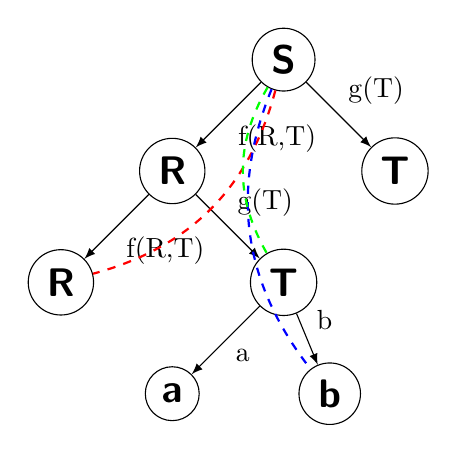
\begin{tikzpicture}[
      node distance = 2cm,
      auto,
      block/.style = {circle, draw, font=\sffamily\Large\bfseries},
      line/.style = {draw, -latex}
    ]
    
    % Nodes
    \node [block] (S) {S};
    \node [block, below left of=S] (R1) {R};
    \node [block, below right of=S] (T1) {T};
    \node [block, below left of=R1] (R2) {R};
    \node [block, below right of=R1] (T2) {T};
    \node [block, below right of=R2] (a) {a};
    \node [block, right of=a] (b) {b};
    
    % Paths
    \path [line] (S) -- node {f(R,T)} (R1);
    \path [line] (S) -- node {g(T)} (T1);
    \path [line] (R1) -- node {f(R,T)} (R2);
    \path [line] (R1) -- node {g(T)} (T2);
    \path [line] (T2) -- node {a} (a);
    \path [line] (T2) -- node {b} (b);
    
    % DFS, BFS, A* paths (without specific details)
    \draw [red, thick, dashed] (S) to [bend left] (R2);
    \draw [blue, thick, dashed] (S) to [bend right] (b);
    \draw [green, thick, dashed] (S) to [bend right] (T2);
    
    \end{tikzpicture}
    \caption{Illustration of the tree of leftmost derivations.}
    \end{figure}


    % \begin{figure}
    %     \centering
    %     \begin{tikzpicture}[
    %       node distance = 1.5cm,
    %       auto,
    %       block/.style = {circle, draw, fill=orange, font=\sffamily\Large},
    %       line/.style = {draw, -latex},
    %       dashedline/.style = {dashed, -latex}
    %     ]
        
    %     % Legend
    %     \node [draw, rectangle, minimum width=3cm, minimum height=2cm, font=\small] at (0,5) {legend};
    %     \node [font=\small] at (0,4.5) {--- semantic equivalence};
    %     \node [font=\small] at (0,4) {⊔ nondeterministic choice};
        
    %     % Nodes for (A)
    %     \node [block] at (0,2) (A1) {+};
    %     \node [block, below left of=A1] (A1L) {5};
    %     \node [block, below right of=A1] (A1R) {x};
        
    %     % Nodes for (B)
    %     \node [block] at (4,2) (B1) {+};
    %     \node [block, below left of=B1] (B1L) {5};
    %     \node [block, below right of=B1] (B1R) {x};
        
    %     % Paths for (A)
    %     \draw [line] (A1) -- (A1L);
    %     \draw [line] (A1) -- (A1R);
        
    %     % Paths for (B)
    %     \draw [dashedline] (B1) -- (B1L);
    %     \draw [dashedline] (B1) -- (B1R);
        
    %     % ... continue for other nodes and paths ...
        
    %     \end{tikzpicture}
    %     \caption{Refactorings and data structure.}
    %     \end{figure}



    \begin{figure*}[htbp]
        \centering
        \begin{adjustbox}{width=\textwidth}
            \begin{tikzpicture}[level distance=1.5cm,
                level 1/.style={sibling distance=6cm},
                level 2/.style={sibling distance=3cm},
                every node/.style={circle, draw}]
            
            \node at (-9,0) {$\lambda$};

            \node at (-6,0) {$\lambda$}
                child {node {+}};
            \node at (-3,0) {$\lambda$}
                child {node {+}
                    child {node {x}}
                };
            \node at (0,0) {$\lambda$}
                child {node {+}
                    child {node {x}}
                    child {node {x}}
                };
            \node at (3,0) {$\lambda$}
                child {node {+}
                    child {node {x}}
                    child {node {max}
                        child {node {x}}
                        child {node {x}}
                    }
                };
            \node at (6,0) {$\lambda$}
                child {node {+}
                    child {node {x}}
                    child {node {max}
                        child {node {x}}
                        child {node {y}}
                    }
                };
            \node at (9,0) {$\lambda$}
                child {node {+}
                    child {node {x}}
                    child {node {max}
                        child {node {y}}
                        child {node {x}}
                    }
                };
            
            % Second tree sequence (Figure 6)
            \node at (-3,-5) {+};
            \node at (0,-5) {+}
                child {node {pow}};
            \node at (3,-5) {+}
                child {node {pow}
                    child {node {y}}
                };
            \node at (6,-5) {+}
                child {node {pow}
                    child {node {y}}
                    child {node {x}}
                };
            \node at (9,-5) {+}
                child {node {pow}
                    child {node {y}}
                    child {node {x}}
                }
                child {node {3}};
            
            \end{tikzpicture}
        \end{adjustbox}
        \caption{Creation of trees showing the construction process.}
    \end{figure*}
    
    














\newpage
\chapter{Philosophical Ramifications}
Here I want to discuss the paradigms assumed more generally, consider alternatives, and discuss the benefits and limitations of the approach and lastly consider the overarching elusive questions every cognitive scientist thinks about: who am I.

\section{\orange{Language of Thought}}

The idea that the thoughts are constructed by some kind of Language of Thought (LOT), in order to understand and represent our reality has a long history. 
Gottfried Leibniz imagined a \textit{Characteristica Universalis}, a formal language capable of expressing metaphysical concepts \cite{sep-leibniz-logic-influence}.
Jerry Fodor, among many other scholars, continued the development of this hypothesis and proposed that our cognitive processes are akin to computations involving a system of mental representations that can be composed into complex thoughts, akin to how sentences are formed from words according to the rules of grammar \cite{sep-language-thought}. Fodor's theory implies an innate structure underlying human cognition, with systematic, rule-governed operations that manipulate symbols.

\subsection{\red{What is a Symbol? - Semiotics}}
Other things to clarify
\begin{itemize}
    \item What is a symbol (also relate to semiotics but also in the cognitive sense. Something that relates to something else, a pointer. Think of memories that are stored in the hippocampus.) what about bioelectrical prepatterns? are all representations symbolic? How would symbols be implemented in the brain?
    \item Analytic vs. Geometric Solutions as an analogy to approximation vs symbol? imitating understanding vs actual and think about whether there is actually any difference. perhaps a limitation of the symbolic programming approach is that it is rigid and less flexible?
\end{itemize}
\begin{itemize}
    \item Explain the different gradients of symbols. e.g. SPA is symbol-like. Part whole hierarchies and capsules are also kind of a symbol in that there is a central representation of a concept. I think its about centrality vs distributed representation and also about the capabilities of the symbols, i.e. does cognition work by only manipulating the symbols, rather that the representations themselves? What is that extra layer needed for then? Think of SPAs layered vectors, shallow vs deep understanding.
    \item If we argue that the LOT is a kind of a self-organising system, then what are the parts (the primitives) we construct (analogy to primes and how every natural number can be constructed using primes.) What are the primitives here? Do we have some axioms of ontology? Are they built in? I.e. taking the stance that we do not start off with a clean slate (Turing) (inductive biases?). Perhaps through evolution? 
    \item Maybe talk about the idea that concepts might start off simple, i.e. starting with light and dark, warm and cold, then increasing the complexity of concepts, like Hubel \& Wiesel. 
    \item This kinda goes back that every sacchade is a query to the world. Werner Heisenberg “What we observe is not nature herself, but nature exposed to our method of questioning.” 
    \item Relate to poverty of the stimulus
    \item relate to piaget 
    \item model vs model free (we dont just learn chess by watching, we either learn about or try to infer the rules.)
\end{itemize}

\subsection{\orange{Semiotics}}
How can we classify concepts?
Ferdinand de Saussure assumed the sign relation to be dyadic: 
there is the form of the sign, the signifier; 
and its meaning, the signified. 
C.S. Peirce thought the sign relation is triadic: 
there is a sign vehicle (form of the sign, the signifier); 
the sign object (the thing it refers to, the signified);
and the interpretant (subjective interpretation). 
Peirce's signs can be deconstructed into three forms:
Icons
	signs that signify by means of similarity between sign vehicle and sign object
	they have physical resemblance to the signified, like a picture of the signified
Indices
	signs that signify by direct contiguity or causality between sign vehicle and sign object
	E.g. smoke to refer to fire
Symbols 
	signs that signify through a law or arbitrary social convention
	These are culturally learned, like the alphabet or the number “9”


About the grounding problem and semiotics: sure, initially, the concept needs to point to something in base reality but once the concept is formed, it can detach from that pointer, it can then be modulated, composed, recombined, etc. to create another concept or be part of a new concept. That way, the network of concepts does not need to be grounded anymore. It is useful though for the concepts to map to the world in some way. This is useful, not accurate. I suspect that the new concepts will then go through some neural darwinism, memetic competition to find which concepts are useful and which aren't, and they will mutate accordingly. I don’t know if in an Darwinian or Lamarckian sense, though. Also, what is a unicorn grounded to?


\subsection{\orange{Formal Grammar}}
\begin{itemize}
    \item Syntax vs. Semantix
    \item Semiotics
    \item We find that GPT also finds an inherent "semantic grammar" in the data. (but we do it differently)
\end{itemize}

undecidable problems:
\begin{itemize}
    \item \rephrase[inline]{Determining if a context-free grammar generates all possible strings, or if it is ambiguous.
    Given two context-free grammars, determining whether they generate the same set of strings, or whether one generates a subset of the strings generated by the other, or whether there is any string at all that both generate.}
    \item The problem of determining the Kolmogorov complexity of a string.
    \item Planning in a partially observable Markov decision process.
    \item Game of Life
    \item halting problem
    \item polymorphic typed lambda calculus (second-order lambda calculus)
\end{itemize}

% \subsection{Gödel's Incompleteness Theorem and Turing's Extensions}
% \subsection{Chomsky's Hierarchy}
% \subsection{Computational Irreducibility}
% \subsection{Constructivism}
% \subsection{The Notion of a Semantic Grammar}
% Church-Turing Thesis



\subsection{\red{Incompleteness Theorem}}
If our thoughts are indeed composed by some language, we can let our intuitions about its structure and limitations be guided by the advances made in the past century in regards to formal languages and computationalism.
Gödel showed that any formal system strong enough to express Peano Arithmetic is incomplete \cite{sep-goedel-incompleteness}. Turing showed that any possible computation can be done by a Turing machine and concluded that the human mind must be computational \cite{JCopeland2004-JCOTET}. [Piccinini disagrees]


\subsection{\red{Chomsky's Hierarchy}}
Chomsky's Hierarchy classifies formal languages of different strengths and the automata that recognize them \cite{chomsky1959certain}.
Show the mapping of chomsky hierarchies onto the brain, relate it to \cite{dehaene_symbols_2022} showing different DSLs in different brain regions.


Many contemporary versions of the LOT hypothesis (LOTH) argue that our conceptual framework is constructed bottom-up using some initial primitives. More so, the language we construct concepts in is executable, akin to a programming language \cite{dehaene_symbols_2022}. The idea is that we model the world by creating programs that generate our observations \cite{rule_child_2020}.

Roumi et al.'s experiment indeed suggest that humans may interpret and compress sequence regularities in a type of program of minimum description length (MDL) \cite{al_roumi_mental_2021}.
Dehaene et al. further test this hypothesis and find similar results \cite{dehaene_symbols_2022}.





\section{\orange{What is Truth?}}
- semantic closure

% From Donald hoffmann and joscha bach: consciousness , etc. .. : proof cannot reach truth. godel found that there is truth that cannot be found with mathematics. but the opposite is true. there is no deeper notion of truth than proof. perception cannot be true or false. it just is. physical events cannot be true or false, a pattern you observe isnt true or false. the pattern itself is an interpretation. its hermeneutics. in order for something to be true or false you need a language which needs to be defined such that truth can be established. And the process of establishing truth is a computation. There are two types of languages in which truth can be defined: classical mathematics is stateless and thus timeless. it lacks the temporal dimension. this allows you to create functions that take infinitely many args in a single step. but in a computational system you cannot assign a single digit to pi. here, in a language with steps, we are losing the ability to treat pi as a value. it is now a function we can only approximate to a certain degree. we get a fundamental difference between a value and a function. (relate this to the universal function approximator: can we approximate downstream functions? perhaps thats what we need symbols, or grounding for). this means that also truth changes. its no longer this platonic thing that exceeds mathematics . it has to be contingent on the language that uses it. if the language has internal contradictions, truth becomes impossible to determine and you can never prove statements that cannot be described in your language (extrapolation). 

%     In essence it means that we can define languages which do not align with the real world, but are above it. we need to define languages of the same level as actual reality. 


% Proof cannot reach. Gödel found that there is truth that cannot be found with mathematics. But the opposite is true. There is no deeper notion of truth than proof. 

% Perception cannot be true or false. it just is. Physical events cannot be true or false, a pattern you observe isn't true or false. The pattern itself is an interpretation. It’s [hermeneutics](craftdocs://open?blockId=AAA69614-E593-4EAF-8DE7-66B0C6B3F611&spaceId=cbf6d066-0b3e-1851-819b-e530e63289b3). 

% In order for something to be true or false you need a language which needs to be defined such that truth can be established. And the process of establishing truth is a computation. 

% There are two types of languages in which truth can be defined: 


% - Classical mathematics is stateless and thus timeless. it lacks the temporal dimension. This allows you to create functions that take infinitely many args in a single step. 
% - But in a computational system you cannot assign a single digit to pi. Here, in a language with steps, we are losing the ability to treat pi as a value. It is now a function we can only approximate to a certain degree. We get a fundamental difference between a value and a function. 
% 	- (relate this to the universal function approximator: can we approximate downstream functions? perhaps thats what we need symbols, or grounding for). 

% This means that also truth changes. It’s no longer this platonic thing that precedes mathematics. So, the arrow doesn’t go from true states to a language that describes it, but it has to be contingent on the language that uses it. Truth is established by constructing sentences in a language. 

% If the language has internal contradictions, truth becomes impossible to determine. 

% You can never use your language to prove statements that cannot be described in your language (extrapolation).

% The only hope is to capture observations about reality in your language and describe it so well so that you can infer statements that hopefully align with reality. 


% 	- I.e. you create a generative model of the world and make inferences in that generative model.

% Self-referential paradoxes like “This statement is false” are stateless and therefore do not work. The truth predicate will fluctuate/ oscillate between true and false 

% This is the same discovery Turing made with the 

% Only a thought can be true or false (assuming that there is objective truth (not sure if thats the case. see Levin for ”observer dependent cognition/ computing” and [the universe is not locally real](craftdocs://open?blockId=ABFD3343-79B6-4BDE-AEC3-51010DE306C4&spaceId=cbf6d066-0b3e-1851-819b-e530e63289b3). Gödel’s theorem is rooted in Peano arithmetic and we then must ask, does mathematics exist? and is it absolute? here we always need axioms.

% We established that perception is generative, we create the world as we observe it and thus we never really have access to physical reality but only to our model of the world, these somatosensory perceptions are the axioms we build our world model on. But these axioms are already biased, since we generate them, i.e. perception and generations are inseparable.

% Popper noted that in order to find epistemological truth, statements must be **falsifiable.** But paradoxes like “This statement is false”, because of its self-referential nature, are not falsifiable. 

% It is correct that our models of the world allow for generalisation, i.e. we can imagine things that are not actually possible (e.g. creating a paradox). This is also true of mathematics itself. It is a language which can describe things that are not implementable.   
% But contrary to the usual interpretation of Gödel’s theorem, these super-statements, i.e. statements that describe the non-implementable are not true in the same sense that implementable statements are.

% Only an interpretation can be true or false, thus we need this symbolic abstraction to be able to determine whether something is true or false.

% In that (symbolic?) language, we need to be able to construct sentences. Constructivism! this is the necessity of causal models (i.e. gflownet or similar rather than just transformer)



- David Deutsch: computation is a physical process, thought is a computation, therefore thought is limited by constructive mathematics/ computation, not by pure mathematics.


- constructivism, originality and plagiarism, everything comes from something, there are not isolated events

- computations are physical processes and are therefore restricted/ defined by physics and not by pure mathematics.


% The discourse on the nature of truth in mathematical constructs and perceptual reality draws from Gödel's incompleteness theorems, which delineate the limitations of formal systems in encapsulating all truths. This principle indicates that truth transcends the axiomatic boundaries of mathematics, an assertion that resonates with the tenets of constructivism in philosophy. The dichotomy between classical mathematics and computational systems exemplifies this; where the former is a timeless realm that operates beyond the constraints of sequential computation, the latter recognizes the inherent approximation in the process of computation, as evidenced by the representation of constants like pi. [podcast bach, hoffman]

% Popper's postulate that a statement must be falsifiable to be considered scientifically valid introduces a critical lens through which the nature of truth can be evaluated. This criterion for demarcating scientific theories from non-scientific ones provides a methodological approach to the constructivist perspective, emphasizing the role of empirical refutability in establishing epistemological truth.

% In consonance with Popper's falsifiability criterion, Michael Levin's observer-dependent cognition underscores the subjective nature of perception and its influence on the construction of reality. This aligns with the assertion that truth is not an external, platonic form but a construct contingent on the observer's language and model of the world. As such, the generative nature of perception dictates that our sensory experiences are not passive reflections of an objective reality but active constructions based on internal models and axioms.

% This section posits that the generative aspect of perception necessitates a symbolic language capable of constructing sentences that can encapsulate and convey truth. It suggests that the quest for truth in both mathematical and perceptual domains is not a pursuit of an absolute external reality but a constructive process influenced by the observer's cognitive and linguistic frameworks. The implications of this for the development of causal models are profound, as they require a shift from purely transformational algorithms to those that can incorporate and simulate the generative nature of human cognition and perception.



% This text discusses the philosophical and computational aspects of truth, proof, and perception. It asserts that while Kurt Gödel's incompleteness theorems reveal that some truths cannot be proven mathematically, the concept of truth is nonetheless fundamentally tied to proof within any given language system. The text distinguishes between stateless classical mathematics, which lacks temporality and can handle infinite arguments in a single step, and computational systems that require approximation, as seen with the value of pi.

% The essence of truth is presented as mutable, contingent on the language used to describe it. If a language contains internal contradictions, it becomes impossible to determine the truth. The act of establishing truth is seen as a computational process, and languages must align with observed reality to make accurate inferences. The text mentions Gödel's theorems and Turing's work, which touch upon self-referential paradoxes and the observer-dependent nature of cognition, suggesting that our perception is generative and shapes our model of the world.

% Popper's criterion of falsifiability is invoked to assess the truth of statements, noting that paradoxes cannot be falsified and thus pose a challenge to traditional views of truth. The text concludes that only symbolic languages allow us to construct sentences and determine truth or falsehood, emphasizing the importance of causal models over mere transformational ones in understanding and describing reality.












The question then remains, where primitives actually come from.
\subsection{\red{Where do the symbols/ primitives come from?}}

\subsubsection{\green{Neurosymbolic AI}}
[should this be in the concept section?]

Garcez et al. analyse connectivist and symbolic paradigms and find that the most effective AI would integrate these approaches \cite{garcez2020neurosymbolic}. They find that for effective learning from data, knowledge in neurosymbolic AI should be embedded into vector representations. Once networks are trained, symbols can be extracted. These symbols are not only descriptive but also operate at an optimal level of abstraction. This facilitates infinite applications with finite resources. Furthermore, this enables compositional and discrete reasoning at the symbolic layer, providing the capability to extrapolate beyond the given data distribution. Combinatorial reasoning is challenging. The combination of learning and reasoning addresses this problem by learning to reduce the number of effective combinations. 
Consider a neural network that learns certain regularities and recognizes that whenever it sees features of type A, features of type B are also present, but features of type C are not. This implicit rule can be made explicit by converting it into symbols: $\forall x A(x) \rightarrow (\exists y B(y) \land \lnot \exists z C(z))$.
[relate this to the framing problem that if A and B change, C should change...]


Discussing what LLMs are supposed to model, whether approximations are necessary etc. Symbols. \cite{Blank_2023}

\subsubsection{\red{Variable Binding}}



\section{\orange{What is Meaning?}}
- what do the symbols mean? or "what's all that jazz (for concepts or so)"
- is there a need for symbols?

Conceptual role semantics (CRS) is the view that the meanings of expressions of a language (or other symbol system) or the contents of mental states are determined or explained by the role of the expressions or mental states in thinking. The theory can be taken to be applicable to language in the ordinary sense, to mental representations, conceived of either as symbols in a ‘language of thought’ or as mental states such as beliefs, or to certain other sorts of symbol systems. CRS rejects the competing idea that thoughts have intrinsic content that is prior to the use of concepts in thought. According to CRS, meaning and content derive from use, not the other way round.

\begin{itemize}
    \item variable binding
    \item grounding
    \item binding problem
\end{itemize}

Piantadosi asserts that symbols have no inherent meaning, instead, meaning emerges from the dynamic relations between symbols. I.e., only the conceptual role and the dynamics of the symbols define meaning \cite{piantadosi2021computational}.

By defining meaning as an emergent phenomenon of conceptual roles, Piantadosi and Hill do not rule out that large language models (LLM) already have some foundation of meaningful concepts \cite{piantasodi2022meaning}.

Recent work tries to relate these ideas to biological systems, e.g. Quan et al. propose how role-filler interactions could be implemented in the brain via temporal synchrony to permit symbolic processing and dynamic binding of variables \cite{do2021neural}.

Santoro et al. argue for a semiotic approach, assert that symbols are subjective, and propose that meaning of symbols in artificial systems will arise when they are subjected to socio-cultural interactions \cite{santoro2021symbolic}.





Meaning: You establish the relationship between pattern and the function that describes the universe, your conceptual model, and that is meaning. Meaning is your entire mental universe. It's the unified model of reality that your mind is constructing. So for any new thing, if we can establish a relationship between the thing and our model, it has meaning. If we can place it in our conceptual framework, it gets meaning. 

- subsubsection: what is meaning?

\improvement[inline]{difference between what is meaning and what is meaningful, maps of meaning. what is meaningful is what guides you. its a gradient, a heuristic. Show studies that deeper understanding improves memory and meaning.}





Ellis et al. use $\lambda$-calculus, which is Turing complete, to build something akin to a LOT \cite{ellis_dreamcoder_2021}. In response, Piantadosi shows that combinatorial logic is equivalent to $\lambda$-calculus and why combinatorial-logic-like (LCL) language is preferable, for one because it doesn't assume primitives, thereby avoiding the problem of their meaning and origin.

One of the questions regarding a LOT is whether thoughts can be produced by simple syntactic symbol manipulation.
I (and many others) suspect that semantics are not just an emergent phenomenon but that it actively shapes our perception and concept formation \cite{santoro2021symbolic, hofstadter_gdel_1979}.

Moreover, purely symbolic attempts, albeit being the original approach of artificial intelligence, have proven to be insufficient \cite{garcez2020neurosymbolic}. Instead, the successes of modern AI are owed to the advances of connectionist models. These however, have their own deficits, namely, being incredibly data-hungry, lacking causality, and lacking out-of-distribution generalization, to name a few. Therefore, new approaches try to combine these two AI strands into what is known as \emph{neurosymbolic AI} \cite{garcez2020neurosymbolic}.




\subsubsection{\green{Poverty of the Stimulus}}
\todo[inline]{should this be here?}

The "poverty of the stimulus" argument is an argument that is often made in the field of linguistics and cognitive science. It argues that children are able to learn language despite being exposed to a relatively limited amount of data, which suggests that they must have some innate knowledge or ability that helps them learn language.

The argument is based on the observation that the linguistic input that children receive is often incomplete, ambiguous, or inconsistent. For example, children may hear sentences that contain errors or that are not grammatical. Despite this, children are able to learn the rules of their language and use them to produce and understand sentences that they have never heard before.




\subsection{\orange{Abduction}}
\begin{itemize}
    \item frame-problem
    \item IBE + abduction
    \item Markpoel 7 criteria
    \item Approximation?
\end{itemize}

Blokpoel et al. distinguish seven properties a computational model of abduction proper must conform to, namely isotropy, open-endedness, novelty, groundedness, sensibility, psychological realism, and computational tractability \cite{blokpoel2018deep}. 
\subsubsection{\green{Abduction Proper}}

Abduction proper relates to the \textit{generation} of hypotheses. In DreamCoder, this happens in the waking phase of the algorithm. When confronted with a task, DreamCoder comes up with the $k$ best candidate hypotheses \footnote{Note that I will use hypothesis and program interchangeably, as when speaking about an hypothesis we mean a possible explanation to a problem, which in this case takes the form of programs.}. It does so by enumerative search under the recognition model $Q$. The neural network guides the search by pointing to the branches that are most likely to contain the programs to solve the task, thus narrowing the breadth of the search tree. In other words, branches of unpromising programs are being eliminated.
By enumarative search using the recognition model, programs are chosen that are both the likeliest as well as the most succinct. The result is that programs are returned, enumerated by their posterior probability.

In the following I will go through the seven properties of abduction proper as outlined in Blokpoel et al. \cite{blokpoel2018deep} and compare them to the implementation in DreamCoder.

\paragraph{\green{Isotropy}} Fodor denotes that any knowledge that the system has, might be relevant to the solution of the task and should therefore be accessible \cite{fodor1983modularity}.
DreamCoder does adhere to this principle, since all the knowledge it has is encoded in its library which is accessible in its entirety when generating hypotheses. Therefore, if a sub-program is relevant, it can be included in the proposed program. 

\paragraph{\green{Open-endedness}} The set of candidate hypotheses should be open-ended, meaning that it can contain any hypotheses which one could in principle infer. Here too, DreamCoder abides by the principle. All the programs that solve the task $x$ could in principle be included by the set of candidate programs. The authors set the number of candidate hypotheses to $k = 5$ for efficiency. However, one could also list all candidate hypotheses without restrictions.

\paragraph{\green{Novelty}} An agent should be able to generate novel hypotheses, i.e. programs that are not already stored in the library. In DreamCoder, programs are represented as polymorphically typed $\lambda$-expressions which allow for the ability to define new functions. When presented with a (novel) task, DreamCoder synthesizes programs, tailored to the task. This is one of the main features of the algorithm: program synthesis.

\paragraph{\green{Groundedness}} A candidate hypothesis should be grounded, meaning, the relation of the representations of the explanandum and explanans should be well-defined. Since DreamCoder uses a DSL, this property is inherent in the system. Moreover, the output of DreamCoder is a library of programs (along with a recognition model). Programs are universal and can be represented by any Turing-complete language.

\paragraph{\green{Sensibility}} A candidate hypothesis should explain the observation. All candidate programs suggested during the wake phase are sensible, as they are only selected during search if they solve the task at hand. 

\paragraph{\green{Psychological realism}} The computational mechanism which supports abduction proper should be biologically plausible. This property however, matters only if human abduction proper is to be replicated or studied. To study the mechanism itself this property is not a necessity. In any case, the wake-sleep algorithms is heavily inspired by our own sleep cycles and Lewis et al. show a remarkably similar finding in the human brain, interestingly using the same example of the analogy between an atom and a solar system used in Blokpoel et al., and previously Gentner in her original Structure-mapping Theory \cite{lewis2018memory,blokpoel2018deep, gentner1983structure}.

\paragraph{\green{Computational tractability}}
Search is done by a specifically engineered parallel enumaration algorithm which combines Best-first and Depth-first search which run with $\mathcal{O}(n)$ and $\mathcal{O}(\log n)$, respectively. Hence, given the library, as well as the trained recognition model, abduction proper actually becomes tractable.




\subsubsection{\green{Inference to the Best Explanation}}
Now that we already have a set of candidates, how do we select the best of the generated hypotheses? After applying neurally guided search, we have an enumerated list of programs solving the task. \textit{Best} is defined in DreamCoder as the shortest program with the highest probability of solving the task. This makes it seem as if abduction is solved easily and tractably. However, the bulk of the computations happen in the sleep phases. In the dreaming phase, the recognition model $Q$ is trained to solve MAP inference, on both replays and fantasies and it is known for MAP inference to be NP-hard. Nonetheless, in replays the system only marginalizes over the best $k$ programs for each task, which reduces the amount of computations and makes the model scalable. 
One of the major hinderences in the quest for commonsense in AI is the problem of finding the \emph{relevant} pieces of knowledge while ignoring irrelevant information \footnote{For an extensive discussion on the frame problem, see \cite{haselager1997}}.
There are two main approaches trying to solve this problem. One is to improve the representation of the knowledge while the other posits a better inference should be applied. DreamCoder implements both these strategies; in fact, these two approaches bootstrap each other and keep improving while learning new tasks.

\paragraph{\green{Representation}} Regarding the representational approach, the question arises of how implicit knowledge should be dealt with. Say, $A > B$ and $B > C$, implicitly we know, $A > C$. This piece of information though, has to be derived before it can be used. Similarly, once this has been derived and has been made explicit, if any of the relations change, it might happen that a derived conclusion has to be adjusted retrospectively. This opens up new problems. One way of solving this is by using intrinsic representations which means that the representations of the relations have the same constraints as the actual relations \cite{palmer1978fundamental}. 
In DreamCoder knowledge is represented symbolically, i.e. the programs in the library are implemented as syntax trees. During the abstraction phase, programs that have been found during wake are refactored. The authors leverage \emph{E-graph matching} which is a data structure that can compactly represent alternative versions of the same program and \emph{version space} which is a data-structure that allows for efficient set operations on its compactly represented programs, to deal with the combinatorial explosion that arises with refactoring. In essence, during abstraction the system looks for sub-routines that have been useful across many of the existing programs as well as the programs that have been newly found during wake and compresses them into new concepts which can be used in upcoming tasks. In this way, explicit knowledge is made more accessible and although the overall library grows, the depth and breadth of the library virtually shrinks because many sub-programs that are deep in the library don't have to be used anymore. Moreover, crucial implicit knowledge is therefore inferred and made explicit. Since the system develops and learns over time, it can adapt whenever it encounters novel tasks.

\paragraph{\green{Inference}} Proponents of the inferential approach usually don't dismiss the symbolic representations but propose that developments in order to better understand inference itself must be made. This is exactly where IBE comes into play. During dreaming, DreamCoder strengthens the mapping between programs and tasks during \emph{replay} and during \emph{fantasies} it learns to deviate from the observed data-set. This means, that the system learns to quickly recognize which patterns in the library are useful and how to quickly find them. One could say, it learns an intuition for the task-domain. It can therefore extrapolate to new tasks.

During waking then, DreamCoder has an improved library of programs, as well as a better recognition model to navigate it. Crucially, this dual bootstrap between the two modes is what catapults the learning of the domain. An improved library with better abstractions and concepts leads to a better and more efficient usage of it which leads to better programs which can be found which in turn can be abstracted further. 


\begin{itemize}
    \item induction, deduction, abduction, inference to the best explanation
    \item "Although it is not clearly understood by many, classic grounded theory utilizes deduction, induction, and abduction as the necessary logic functions of the research process. Glaser’s described the forms of logic—induction, abduction, and deduction—but referred to them as conceptualization, theoretical coding, and theoretical sampling. Induction begins with data and produces concepts, which are the building blocks of grounded theory. Employing abduction, the analyst infers relationships among the concepts to develop interrelated hypotheses. Deduction is used to gather data to fill in the gaps and produce an explanatory theory. Each type of logic is indispensable to classic grounded theory method. The purpose of this methodological paper is to briefly describe the process and product of each type of logic as applied to the language and procedures of classic grounded theory. - The Logic and Language of Classic Grounded Theory: Induction, Abduction, and Deduction" [is this related to the way concepts share information and are constructed? top down (deduction), bottom up (induction), lateral (abduction), maybe not because different truths are established? check this]
\end{itemize}


\subsection{\red{Subsymbolic Parse Trees}}
Implicit vs explicit
\begin{itemize}
    \item GLOM also related to NCA and to holarchies
    \item Kissner
    \item JEPA
    \item etc. 
    \item other world models, schidthuber, etc.
\end{itemize}









\section{\orange{What Is a Computation?}}

\subsection{\orange{Computational Mind}}
\begin{itemize}
    \item RNA computation [paper]
    \item LCL, etc.
    \item Church-Turing Thesis
    \item Difference in computation between brain (Piccinini), ANNs and symbolic processing
    \item Is computation the only way to truth (relate this to constructivism)
    \item computational irreducibility: we can use generative models as a shortcut sometimes. we can compress regularities. But Wolfram shows that sometimes that is impossible. if truth is whatever is computable, and we take note of the idea of computational irreducibility, it means that there are some computations in which we must apply every step to get there. there is no shortcut. 
\end{itemize}

\begin{itemize}
    \item Do we have one generative model or multiple competing models (multiple DSLs, trying to find the best one)? Or do we just have competing representations at the frontier and it is more difficult to change beliefs deeper in the conceptual space, where concepts are foundational and others rely on?
    
    \item Jerome Busemeyer uses Quantum formulations to show how we are in a super-position of beliefs until we collapse them upon evidence. 
\end{itemize}












\section{\orange{What is a thought?}}
\begin{itemize}
    \item Explain the idea of a thought as a trajectory through semantic space. 
    \item How does this trajectory look like in LLMs? (Wolfram)
    \item How does this trajectory look like in GFlowNet? (perhaps operationalised as a Markovian trajectory?)
    \item How does a thought look like in enactivist/ purely reactive or reflexive cognitive frameworks. 
    \item Thought as constructing probabilistic programs
    \item What does it mean to have a model?
    \item What do we model? Res extensa, Res cogitans. The inside as well as the outside world (Reference Solms, JB, Decartes)
    \item What does it mean to compute?
    \item Can any concept be definitively defined as a particular concept (either symbolic or symbolic vector e.g. SPA, hyperdimensional vectors) or are all concepts approximations?
\end{itemize}













\section{\orange{What Does It Mean to Understand?}}
\subsubsection{\red{Operationalising "Understanding"}}
\begin{itemize}
    \item Reverse Engineering: Is understanding being able to reconstruct the thing we want to understand? If you can break down an object or concept and then reconstruct it, perhaps it implies you understand it.
    \item Modelling: Understanding might be proportional to the model we create of a concept. The more accurate and comprehensive our model, the greater our understanding.
    \item Utilization: It could also be the degree to which we can use a concept. If we can apply it effectively, we could claim to understand it.
    \item Maybe understanding is the size/ strength of a concept? Imagine it as blobs in an abstract space, a large blob with many connections would be understood, whereas a new little blob with little connections is not. 
\end{itemize}



What does it mean to truly understand something? 

I would say that understanding requires causality, not just correlation. (Searle's chinese room)


Is it possible for artificial intelligence to grasp the essence of a concept like “body” or “mass”? It can approximate to an arbitrary degree but you can't square the circle, i.e. approximations at the limit do not become the thing approximated, they are just treated as such. This is related to joscha bach's interpretation of Gödel's theorem, that it cannot be implemented since there are no infinities in physical reality. Anyways, approximations might be enough, and might be what we're doing too. This is important for the symbolic vs connectionist debate.

GPT learns through the context in which words and phrases appear, essentially creating a concept network of words. The AI analyses this abstract relational structure to generate responses. Yet, we might question whether this process equates to understanding.

The conundrum is reminiscent of the mary's room thought experiment, in which Mary, despite having all the data about colour, has never truly experienced it. If she were to experience colour one day, would she glean any new information that was not already available in the data she had studied?

The question seems to probe whether phenomenological experience can be simulated through abstract data. While it's possible to argue that a blind man will never truly see just by reading about it (in braille), we must also consider that our experiences are essentially the result of neurons firing in our brains. If we possess the necessary cognitive mechanisms, it's plausible that phenomenological experience could be replicated by alternative means.











































































































\section{\orange{What is a Concept?}}
\subsection{\red{Identity and Essence}}
How do we discern between things?

Here we discuss homeostasis, allostasis | me against the world
\subsubsection{\orange{Categories}}
\begin{itemize}
    \item Prototype Theory ( + prototype, stereotype, archetype) (types and relation to programming?)
    \item intension extension?
    \item In LLMs concepts are defined by the way they are used. By correlation. By function. It could be defined by its properties, by its causal function, etc. 
    \item LLMs
    \item mereology
    \item ontology
\end{itemize}

\begin{itemize}
    \item substance theory
    \item process theory
    \item krakauer information individuality
    \item Relationship between agent and environment. Embeddedness, we are inseperable; Üexküll called this bio-semiotics and the extended phenotype (the spiderweb is part of the spider, humans domesticated fruit, animals, etc. these are all part of what it means to be human.)
\end{itemize}




\subsubsection{\orange{Computational models of categorization}}

In their study, Zeithamova et al. delve into two predominant models of concept representations: \gls{prototype models} and \gls{exemplar models}. The former views categories as generalized representations where category membership hinges on an object's similarity to a prototype, while the latter represents categories through specific exemplars, basing membership on an object's similarity to these stored exemplars \cite{zeithamova_brain_2019}. Their findings suggest that during concept learning and category processing, high-level abstractions, such as associating an airplane with a car due to their shared role in transportation, are processed in the dorso-lateral pre-frontal cortex, associated with $\beta$ oscillations and bottom-up processing. On the other hand, low-level abstractions, like identifying a new cat based on prior knowledge, are linked to the ventro-lateral pre-frontal cortex, involving $\gamma$ oscillations and top-down processing—this latter approach resonating more with object-recognition or pattern-matching challenges.

\improvement[inline]{relation to FEP, generative model, sys1,2 etc.}

Feature-based models: These models represent categories as a set of defining features. They assume that category membership is based on the presence or absence of specific features.

Connectionist models: These models represent categories as patterns of activation in a neural network. They assume that category membership is based on the pattern of activation that results from processing sensory input.

Bayesian models: These models represent categories as a probability distribution over features. They assume that category membership is based on the likelihood that an object belongs to a particular category given its features.

- I think categories, similar to any self organizing system maintain a boundary of what they are and what they are not. they themselves can be thought as agents. We have the concepts but our perceptions are shaped, mostly by evolution and society. Our subjective interpretation is actually minimal. Our perception of objects strengthens in concordance with the crowd, the society. So these concepts, which are sort of memes can be seen as agents themselves. They self-organise, and have a mapping to the actual underlying brain structure which is a mapping of the environment, to solve certain problems. a concept is the minimization or optimization of free variables in an active inference frame. This relates to gibsons affordances. so concepts might be formed also by function, or the relation of how i could interact with the concept. but concepts dont always have to be functional. this is also related to meaning. the function of a concept is its meaning. in that way it is the set of inferences one could make from said concept. of course it doesnt mean that it is meaningful, which is subjective to the observer and dependent on personal preference and goals. concepts are agents that serve a goal. notice how concepts have different levels of granularity, according to our interaction with them. 







\subsection{\orange{concepts}}




\begin{itemize}
    \item is a concept a symbol? 
    \item Do concepts exist?
    \item JBs interpretation
    \item Semiotics
    \item Symbolic vs distributed representation of symbols
    \item Are concepts discrete or continuous (symbol vs connectionsim)
    \item Do concepts exist?
    \item Is the self a concept?
\end{itemize}


\begin{itemize}
    \item the transcendentals as the axioms of ontology (what are the eigenvectors of cognition?)
    \item proto-concepts
    \item concepts vs no concepts
    \item concepts as pointers
    \item normalizing over sensory data -> features -> objects -> concepts 
    \item Concepts could be "chunked" into hyperdimensional vectors
\end{itemize}

\subsection{\orange{How do concepts form}}
- Concepts are the address space of mental representations. They are merely pointers. 
- There's a hierarchy (holarchy) of abstraction of mental representations
- The least abstract thing are impulses that come from sensory neurons. 
- Basically, discernible difference, which is how we define information, is the closest to physical reality.
- We organize them into features. features describe how reality changes in the aggregate from moment to moment.
- Features are arranged into objects
- Objects remain stable if the perspective changes
- Concepts abstract over all objects that belong to a group - the extension of a category
- These concepts are organized in an embedding space  



% [rewrite the following]
% Concepts are the address space of mental representations; they function as mere pointers within the vast repository of the human cognitive landscape. By delving deeper into the hierarchical nature of these mental representations, we can elucidate the progression from sensory experiences to abstract concepts and the intermediate stages in between.

% At the most fundamental level of this hierarchy are the impulses emanating from sensory neurons. These impulses are the least abstract entities in our mental representation structure. They provide us with raw, unfiltered data about the external world. This data, in its crudest form, captures the discernible differences in our environment. The notion of discernible difference is pivotal, as it is through these differences that we essentially define information. This level of representation is the closest we get to the physical reality, offering us a window into the objective world.

% As these sensory impulses flood our cognition, the brain begins the task of organization. Here, we witness the emergence of features. Features are holistic descriptors that capture how reality undergoes changes from one moment to the next. They aggregate the nuances of discernible differences, creating a richer, more comprehensive picture of our surroundings.

% In the subsequent tier of abstraction, these features coalesce to form objects. The stability of objects is a testament to their resilience: even when our perspective undergoes shifts, these objects retain their essence, serving as anchor points in our perception of reality. This stability allows for consistent recognition, facilitating efficient cognitive processing and interpretation of the environment.

% As we ascend further in this holarchy, we find that objects serve as the bedrock upon which concepts are constructed. Concepts are abstract generalizations that span across all objects belonging to a particular group. They define the extensions of categories, grouping similar objects based on shared attributes or functions. Rather than focusing on individual instances, concepts provide us with a broader, more generalized view, allowing for efficient cognitive navigation.

% Lastly, these concepts, with their diverse range and depth, find their place within an embedding space. This space organizes concepts in a manner that reflects relationships, similarities, and differences. By mapping concepts within this embedding space, the human brain can easily traverse from one idea to another, drawing connections, making inferences, and expanding upon existing knowledge.

% In conclusion, the journey from sensory neurons to conceptual structures is a testament to the brain's ability to organize and abstract information. Through a well-defined hierarchy, the mind seamlessly transitions from raw data to intricate, abstracted concepts, enabling us to perceive, understand, and interact with our world in meaningful ways.














































Conceptual space (relate this to Gordenford)










\subsection{\green{Semantic Pointer Architecture}}
Eliasmith et al. propose Semantic Pointers (SP) as neural representations that carry semantic content and can be thought of as vectors in high-dimensional space. They are composable into the representational structures necessary to support complex cognition \cite{eliasmith2013build}. To illustrate the notion of SPs, see figure \ref{fig:sp}. On the left we see how a visual percept, in this case a table, is compressed sequentially, much like in the layers of the visual cortex to eventually be represented by a single vector - a semantic pointer. 
    On the right we see the "inverse" function in which a semantic pointer is decompressed and returns the table. Notice that due to noise, the result does not correspond exactly to the original input. 

\begin{figure*}
    \centering
    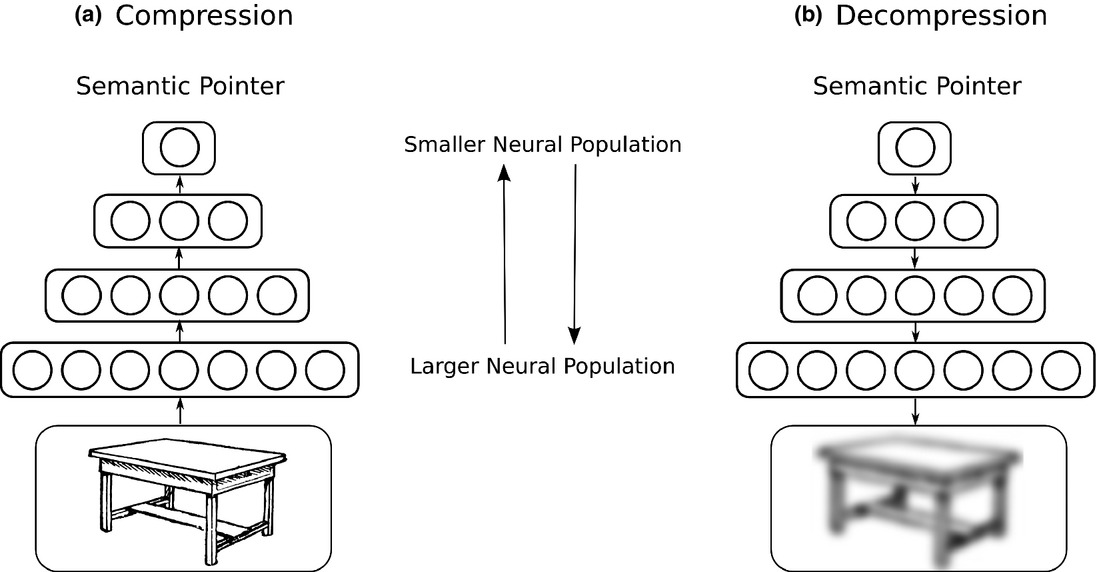
\includegraphics[width=\textwidth]{../img/semPointer.jpg}
    \caption{(a) A sensorimotor input, here a table, is compressed sequentially into a Semantic Pointer. (b) A Semantic Pointer is decompressed and returns a representation of a table. Due to the compression process the decompression results in noise. The figure is taken from Blouw et al. \cite{blouw2016concepts}.}
    \label{fig:sp}
\end{figure*}















































\subsection{\green{Concept space} \label{subsec:gaerdenfors}}
\story{Properties of concepts, introducing the idea of concepetual spaces and a geometry of concept space (latent space)}

Gärdenfors offers a geometric interpretation of cognition that serves as a bridge between the sub-symbolic and the symbolic, between the perceptual and the conceptual \cite{Gaerdenfors}. Her argues that concepts can be represented as regions in a conceptual space, where the dimensions of the space correspond to the different features or properties that can be used to describe the concepts.

In this model, each quality dimension — be it temperature, weight, brightness, or hue — becomes an axis in a multi-dimensional space. Concepts are then regions within these spaces. Imagine, if you will, a three-dimensional space where color is represented: one axis for hue, another for saturation, and a third for brightness. A "concept" like 'red' would be a specific region in this 3D color space.


In mathematical terms, a set is convex if, for every pair of points within the set, the line segment connecting them is also contained within the set. Imagine a balloon. If you pick any two points within the balloon and draw a line between them, that line never leaves the space of the balloon. In Gärdenfors' geometric concept space, most concepts are "convex" regions. For example, if you have a swan and a goose and consider them both as instances of "bird", then it's likely you'll consider everything in between also a "bird".


[expound on that, and relate to rest]

% Peter Gärdenfors' theory of conceptual spaces is a geometrical framework for representing and reasoning about concepts \cite{Gaerdenfors}. Gärdenfors argues that concepts can be represented as regions in a conceptual space, where the dimensions of the space correspond to the different features or properties that can be used to describe the concepts.

% For example, the conceptual space for colors might have dimensions for brightness, saturation, and hue. The conceptual space for animals might have dimensions for size, weight, and diet.

% Gärdenfors proposes that natural concepts are typically \emph{convex}. This means that any two points in the convex region are connected by a line that lies entirely within the region.

% Gärdenfors argues that the convexity constraint is important for a number of reasons. First, it allows us to reason about the relationships between concepts in a natural way. For example, we can say that the concept "red" is more specific than the concept "color" because the convex region for red is contained within the convex region for color.

% Second, the convexity constraint allows us to model a variety of cognitive processes, such as categorization, reasoning, and analogy. For example, we can say that an object belongs to a category if it is located within the convex region for that category.

% Third, the convexity constraint is consistent with our perceptual and motor experiences. For example, the convex regions for colors correspond to the different ways in which we perceive colors.

% Gärdenfors illustrates the idea of convexity with the following example:

% Imagine a cone, where the base of the cone represents the concept "bird" and the apex of the cone represents the concept "robin." All other birds, such as penguins, eagles, and sparrows, would fall within the cone.

% This is because a robin is a more specific type of bird than any other type of bird. In other words, all robins are birds, but not all birds are robins.

% Gärdenfors argues that some concepts, such as "tall" and "short," are \emph{concave}. This means that there are two points in the convex region that are not connected by a line that lies entirely within the region.




% Conceptual spaces are a theoretical framework for understanding how humans represent and reason about concepts. The framework was developed by Peter Gärdenfors in the 1980s and 1990s, and it has been highly influential in the fields of cognitive science, cognitive linguistics, and artificial intelligence. \source[inline]{reference his book}

% Gärdenfors defines a conceptual space as a geometric space where concepts are represented as points or regions. The dimensions of the conceptual space correspond to the different features or properties that can be used to describe concepts. For example, the conceptual space for colors might have dimensions for brightness, saturation, and hue.

% The geometry of the conceptual space allows us to reason about the relationships between concepts. For example, we can define the distance between two concepts as the distance between the corresponding points or regions in the conceptual space. This allows us to measure the similarity between concepts, as well as the degree to which one concept is more specific than another.

% Gärdenfors argues that conceptual spaces provide a powerful framework for understanding how humans represent and reason about concepts because they are:

% Expressive: Conceptual spaces can be used to represent a wide range of concepts, including concrete concepts (e.g., colors, shapes), abstract concepts (e.g., love, justice), and even relationships between concepts (e.g., father-of, above).
% Natural: Conceptual spaces are grounded in our perceptual and motor experiences. For example, the dimensions of the conceptual space for colors correspond to the different ways in which we perceive colors.
% Flexible: Conceptual spaces can be used to model a variety of cognitive processes, including categorization, reasoning, and analogy.

\source[inline]{Gardenfords book (2004)}




I suspect that we use symmetry as an inductive bias [relate to dehaene]. The concept of opposites is a type of symmetrical relation where two entities are diametrically opposed on a spectrum or scale. Day and night, hot and cold, up and down — these pairs may help us organize our world into understandable categories. Of course there are many other types of symmetry, which could act as important inductive biases in order to construct a conceptual world model, 
\begin{description}
    \item[Reflectional Symmetry] When one half is the mirror image of the other half. E.g., many human faces or butterfly wings.
    \item[Rotational Symmetry] When an object looks the same after a certain amount of rotation. E.g., a regular pentagon or a snowflake.
    \item[Translational Symmetry] When an object can be moved (or translated) a certain distance and appear unchanged. E.g., wallpaper patterns.
    \item[Bilateral Symmetry] Seen in many animals, where the left and right halves of an organism are mirror images of each other.
    \item[Radial Symmetry] Where symmetry is centered around a central axis, like in starfish or daisies.
    \item[Spiral Symmetry] Seen in objects like shells or certain galaxies, where there's a continuous curve centered on a point.
    \item[Chiral Symmetry] Refers to objects that are mirror images but not superimposable, like left and right hands.
    \item[Time Symmetry] In physics, certain processes are time-symmetric, meaning they can proceed forward or backward in time without violating the laws of physics.
    \item[Scale Symmetry] When patterns look the same at any scale. Fractals are an example of this.
    \item[Oppositional Symmetry] In abstract terms, where concepts have opposites or counterparts, like good/evil, light/dark, or positive/negative.
\end{description} 

\improvement[inline]{isn't that already inherent since ANNs are doing linear algebra? I think the ANNs are capable of finding symmetrical relations but it could be a more explicit inductive bias/ heuristic? like we see that LLMs find some relations (man : king :: woman : queen), but it could be used explicitly for the construction of concepts. Also think about relational }
[insert figure]




















\subsection{\orange{Hemispheric Lateralisation}}
\begin{itemize}
    \item notion that if we don't have a concept for it, it does not exist for us. I.e. even if our sensory equipment can in principle take it in, and does take it in, it is not there for us. It seems we are unable to attend to it. Perhaps attribute meaning to it and therefore it doesn't enter our conscious awareness.
\end{itemize}

- refer to Wittgenstein, Alfred Korbinszky, etc. analogy with chess

\info[inline]{argument for hemispheric lateralization}
\begin{itemize}
    \item Broad vs narrow attention. One sees the trees, the other the forest.
    \item the left wants to jump to conclusions and is much more quick and dirty, while the right says hang on
    \item left deals with things that are known, when something isn't, its better to leave it to the right until it can be categorised by the left
    \item things in the left are more isolated, while in the right everything is connected to everything else
    \item left is static, right is flowing and changing
    \item the left abstracts, the left is more interested in categories, the right in the unique case
    \item the left sees things as inanimate, the right sees them as animate
    \item as we age we use the representations of what we know increasingly, neglecting the world. We become more solipsistic. This makes sense because perceiving things for the first time is computationally heavy and expensive, so the things we know from experience will usually be good enough.
    \item Talk about confabulation (and perhaps in relation to LLMs)
\end{itemize}

Often, the most obvious things, once unpacked, reveal the most [examples?]. Our most basic perceptions and assumptions are so deeply integrated into our cognitive processes that they become invisible to us, essentially automatic. When driving the same route everyday, people may arrive at their destination without conscious awareness of it. Tasks become automated. [show studies, other examples like piano.]

From a computational standpoint, one could say that these deeply embedded perceptions function much like 'compiled code' in a computer program — efficient and fast, but not easily inspected or altered. These perceptions are model-based representations optimized for computational efficiency, trading off flexibility for speed. They exist as pre-computed "shortcuts" that enable us to interact with the world without incurring high computational costs each time we encounter a familiar situation.

In machine learning, this relates to the trade-off between model-based and model-free learning. Model-free approaches require higher computational costs upfront but are more adaptable. Model-based strategies offer efficient but rigid ways to interact with the world. Both strategies have their pros and cons, reflecting a trade-off between computational efficiency and cognitive flexibility. [source]

As we age, we rely increasingly on these internal representations instead of engaging directly with external reality, making our view of the world more solipsistic. [source]

\improvement[inline]{think of two types of intelligences (crystal vs fluid ?), also exploration exploitation}
\improvement[inline]{We can also include barbara oakley on types of focus, deep and direct, vs broad}

This phenomenon can be explained by the increasing reliance on "cached" or "memoized" cognitive models, which offer a computationally cheaper way to navigate reality. It's a form of cognitive "greedy algorithm," opting for local optimizations based on past experience rather than recalculating the optimal path each time. [source + relation to predictive coding paradigm]

This concept parallels the notion of "overfitting" in machine learning, where a model becomes so tailored to the training data that it loses generalizability. In human cognition, an over-reliance on established mental models could result in decreased adaptability and an insular worldview, effectively isolating the individual from the ever-changing external environment.

As we automate more cognitive functions—either through learned habits or technological aids—we engage less in "active sampling" of the world, reducing the richness and nuance in our perceptions. This leads to a form of "lossy compression" of reality, where only the most salient features, according to our models, are retained.


- Problems should be solved at the lowest possible level of the hierarchy. Larger goals require more sophisticated organization.
- How does a system recognize that it cannot solve it alone and that it needs to recruit other cells? Think of the computational boundary. Perhaps we must be able to estimate computational complexity. 
- This compression of sensory information into concepts may be the origin of symbolic processing. 

- Things we don't have concepts for don't exist. We can't describe them in our language. [related to joscha about truth.] 





% \section{Spaces in Cognition}
% \subsection{Latent Spaces}
% \subsection{Cognitive and Conceptual Spaces}
% \subsubsection{Peter Gärdenfors's Perspective}
% \subsection{The Geometry of Cognitive Spaces}
% \subsubsection{Hyperbolic Spaces} (aligns with holarchies)

\begin{itemize}
    \item show representations in human brains and argue why the brain may largely be a generative model. 
\end{itemize}

A paradigm, coming originally from Ethology is the idea of reactive agents which have four defined "rules" on which they act (Murphy, 2000). Reflexes are hard-wired responses to certain stimuli. A knee-jerk reaction. Taxes
define the movement of an organism towards (or away from) a certain stimuli. An example is the way ants follow a trail by chemotaxis. More complex behaviour is elicited through fixed-action-patterns. These consist of a sequence of certain behaviours, usually triggered by some stimulus. A squirrel's nut burying behaviour is an example. Lastly, the sequencing of innate behaviours such as a digger wasp's brood-tending is an example of even more complex behaviour. Further, it has been shown how complex behaviour can emerge as an epiphenomenon such as in swarms, ants (Franks, 1989) or even in Conway's popular Game of Life (Conway, 1970).



\begin{itemize}
    \item Efficient inference over hierarchical Bayesian models is still difficult.
    \item Approximate inference
    \item Here we can go into models monte carlo e.g. etc.
    \item Einstein: intuition, rationality
\end{itemize}


































































































































\section{\green{Cognition, Nested Multi-scale Hierarchies, and Self-Organisation}}

Biological systems demonstrate remarkable complexity through self-organization, a process where spontaneous pattern formation results from the interactions of individual components within an environment. 

Biological organization is composed of nested goal-seeking agents, maintaining operational and organizational closure through homeostasis and allostasis \cite{ciaunica_nested_2023, vernon_embodied_2015} [explain terms in more detail, or is glossary enough?].

Atoms form molecules, which form cells, tissues, organs, organisms, groups, societies, civilizations, and so on. Levin describes this as a multiscale competency architecture, which is not only structural but also functional \cite{Levin_2023}. Each level of this organization has some competency and solves problems in its own action space. Moreover, each level interacts with the levels above and below which is reflected in the idea of circular causality \cite{ciaunica_nested_2023, vernon_embodied_2015}. 
% Douglas Hofstadter calls this a heterarchy and gives the example





\section{\green{Who am I?}}
In order to understand who I am, I need to understand what I am not.
What is a cognitive system, how does it emerge and how does it develop.
How does a cognitive system make the distinction between it and the world?

\subsection{\green{The Genesis of Cognition}}

When thinking about the genesis of the self, we can think back to our earliest developmental stage, that of being an unfertilised \gls{oocyte}, and realize that the self gradually emerges from it.

Levin shows that upon scratching a \gls{blastoderm}, it self-organizes into twins or triplets, etc., depending on the amount of scratches. \source[inline]{source}. This demonstrates that the number of selves in an \gls{embryo} is not determined by genetics, but is instead a result of physiological self-organization. The problem of discerning between one's self and the external world is an ongoing, dynamic process that needs to be solved "online". This indicates that our self-concept is ever-evolving, reshaped by new information and experiences.

The ability to pursue goals is a trait that all agents have in common and the size of that goal is a way to classify and compare diverse intelligences, Levin suggests \cite{Levin_2022, levin_computational_2019}.

For example, a single-celled organism may have the goal of finding food and avoiding predators, while a human may have the goal of building a family or writing a thesis about cognition.

\improvement[inline]{is the homunculus is basically an advanced version of this?}
The brain builds a map of proprioception. It's a statistical map over nerves that fire together. When they almost always fire together, they're likely to be close to each other. Homunculus.

Now the way we distinguish between us and other people or more generally, us and the rest of the world, is simply by realizing that my actions lead to changes in my proprioception and other's actions do not. I.e. we perceive a change in the environment and we need to classify whether we produced the change or not. If the change and our sense of self aligns, it's likely we did it.  [elaborate]

In \source[inline]{source} Levin expounds on the idea that the self-organisational process of bodies is fundamentally the same as that of minds.
\improvement[inline]{not only in structure but in representation. i.e. can we show that the imagination, the conceptual world has the same structure as the actual hardware? is the software built by the same principle as the hardware? is it growing simultaneosly? is there an isomorphism?}. 

All bodies are \emph{composed} of a multitude of levels of organisation, from single cells to entire organisms. Each tier of this hierarchy possesses unique competencies and goals, yet collaboratively works towards the organism's overarching objectives.

\Gls{embodiment} is the grounding of cognitive processes in bodily experiences. Bodies are not just passive vessels for minds but play an active role in cognition \source[inline]{Serge paper on embodiment, sensorimotor information} [elaborate]. 

Diving deeper into bodily self-organization, organisms such as axolotls exhibit a fascinating ability. Despite undergoing amputation, they can regenerate their limbs and halt precisely when restoration is complete. This ability, despite the variety of starting conditions and challenges, hints at an inherent bodily blueprint or internal representation. Intriguingly, this map is underpinned by bioelectrical patterns, which play a pivotal role not just in regeneration but also embryonic development.

Expanding on this, Levin notes that there is no marked distinction between neural and developmental tissue in this context. Both comprise ion channels and electrical synapses. In fact, novel techniques have emerged to both interpret and modify these bioelectrical blueprints. \source[inline]{source}

These "blueprints", or more precisely, endogenous bioelectric pre-patterns, guide the cells to arrange in a certain way and by manipulating them, for instance by introducing potassium ion channel RNA, Levin and his team successfully induced cells to form eyes in non-ocular locations. More impressively, in the absence of sufficient cells, the system recruits additional cells to realize this goal.

In one experiment, the team modified the bioelectrical pattern of a planarian to have a two-headed form. Upon injury, the planarian regenerated, aligning with this new, dual-headed pattern. This reveals, that the planarian is able to have a representation of a body state, different from its current state. It means it has a rewritable memory and is able to represent \gls{counterfactual states}.

This finding suggests, congruent to the conventional view, that genetic information alone doesn't solely dictate the form and function of organisms. Instead, bioelectric signals play a pivotal role in guiding cellular behaviors and tissue outcomes. Traditional genetics emphasizes the idea that the DNA sequence encodes the necessary information to produce an organism's phenotype. While this is fundamentally true, there seem to be other layers of information that can guide tissue organization and even regeneration.

\improvement[inline]{
This may be a primitive precursor to symbolic thought. Perhaps even to visualization and imagination.
Perhaps moving from bioelectrical pattern representation of the brain, which is in a sense the first counterfactual, this may be the first primitive version of symbolic? representation, and allude to the brain being a machine to store more complex patterns. 
}

\todo[inline]{Show the work of Lenia, how they do it, and what they have achieved. Also, the Gecko thingy from Distill.pub}


\subsection{\green{Computational boundary of the self}}
Levin introduces the term \gls{cognitive light cone}, which metaphorically describes the limits of an agent's knowledge and ability to act. It is defined by the set of all events that an agent can perceive, measure, and model. 
\improvement{introduce cognitive light cone and include stuff from computational boundary of the self}

\subsubsection{\green{Body Patterning and Cognition: A Common Origin}}

Cells are able to make group decisions and regrow into defined patterns.

There is a strong metaphor between “adaptive whole organism behavior and the plasticity of cellular activity during construction and repair of a body”

“Neural networks control the movement of a body in three-dimensional space; this scheme may be an evolutionary exaptation and speed-optimization of a more ancient, slower role of bioelectrical signaling: the movement of body configuration through anatomical morphospace during embryogenesis, repair, and remodeling”

\subsubsection{\green{Multicellularity vs. Cancer: The Shifting Boundary of the Self}}

While healthy cells within a multicellular organism orchestrate their functions to achieve systemic homeostasis, cancerous cells behave in a manner that one might describe as "narcissistically individualistic," focused solely on their own objectives.

In standard physiological states, cellular networks coalesce to fulfill an overarching agenda—namely, the creation and sustenance of intricate macrostructures. Here, individual cells are subsumed into a collective intelligence, a sort of physiological "hive mind" or "swarm intelligence", directed toward system-level anatomical objectives. Contrarily, in the cancerous state, a cell's conception of its 'Self' is shrunk, both spatially and temporally.

Spatially, cancerous cells find themselves in a state of electrical isolation from their cellular neighbors, impairing their capacity for long-distance information exchange and cooperative action. Temporally, the scope of a cell's prospective planning dwindles: where a healthy cell may operate on a time scale spanning decades, a cancerous cell may focus solely on activities that, though enhancing its own immediate survival, jeopardize the host organism in the near term.

Unicellular organisms or cancer cells are not intrinsically more selfish than cells in a multicellular organism; rather, the "Self" is defined as the boundary of information, in terms of space, time, and complexity, that can pass between the subunits. 

Most biological organisms emerges as a hierarchy of nested "selves," each subject to its own evolutionary pressures and game-theoretic dynamics, at varying scales of organizational complexity.

This conceptualization of a dynamic boundary of the 'Self' has implications that stretch beyond the biological realm, into the study of swarm intelligence. Consider, for instance, a termite colony as a "super-organism," with its own extended physiological and rudimentary cognitive functions. This interplay between patterns of cellular organization and larger sociobiological systems offers a poignant example of the scale-invariance that characterizes cognitive paradigms, equally applicable to cellular communities and animal (and human) societies.

\subsubsection{\green{Defining Individuation From a Cognitive Perspective}}

Levin proposes a definition of an individual based on its information-processing structure and the goals it pursues. A coherent, unified self emerges from the integrated activity of its components that work towards specific goal states. This definition can apply to both biological and artificial agents, focusing on the information processing and goal-directed activity of any given system.

The cognitive boundary of an individual is the most distant set of events that a system can measure and attempts to regulate in its goal-directed activity. Different agents have different cognitive boundaries based on their complexity and abilities. For example, a tick has a smaller cognitive boundary than a dog or a human due to its limited memory and predictive power.

Individuals can exist at different levels of organization, with various, sometimes overlapping goals. This framework can be applied to ethology, artificial intelligence (AI), and artificial life. However, more work is needed to make it practical and applicable in these fields.

The volume of possible cognitive boundaries expands over evolutionary time. Innovations in body structure can drastically increase the cognitive boundaries of viable selves. There may be no upper limit to the size of cognitive boundaries, and it's possible that artificial life, biomedical enhancement, or engineered AI could create beings with much larger cognitive boundaries than humans.

Levin concludes that a potential sequence of evolutionary scenarios for the expansion of cognitive boundaries.
“Thus, physiological connectivity is the binding mechanism responsible for the appearance of larger unified Selves.”

The expansion of cognitive boundaries in the biosphere can be traced through a hypothesized sequence of phases, beginning with homeostasis. Homeostatic persistence allows simple systems to maintain spatial and metabolic integrity, providing the basis for cognitive goals. The minimization of anti-homeostatic stress is a powerful driver for evolutionary innovation, leading to the development of richer biochemical networks and memory systems.

One example of an early memory system is chemotaxis in bacteria. More advanced creatures developed complex learning networks, allowing for associative learning and modularity, which in turn led to the evolution of reactive homeostasis into predictive allostasis.

Sensory machinery in complex animals is based on ancient ion channel mechanisms. As cells organize into multicellular tissues, they can share information and expand their cognitive boundaries. The advent of multicellularity results from the drive to minimize surprise, with multicellular organisms providing more predictable environments for individual cells. This leads to the formation of more complex agents with larger goals.

The transition from single cells to multicellular tissues is facilitated by developmental bioelectricity, which enables the exchange of ionic signals among cells to propagate instructive influence. This has been observed in bacterial biofilms and more advanced cell types. Gap junctions, or intracellular electrical synapses, allow cells to selectively share bioelectric states and implement memory. Physiological connectivity creates larger unified Selves, with bioelectric networks responsible for coordinating cells toward common goals, such as body patterning.

The developmental control bioelectric network shares an evolutionary history with the nervous system, and neurotransmitter molecules are used downstream of bioelectric driving forces. Tunneling nanotubes, axon-like structures with gap junctions at their ends, enable directed connections between cells and pave the way for neural axons and electrical synapses. The bioelectric system was optimized for speed in nervous systems, using the same mechanisms to optimize input-output relations within and between internal mechanisms and the outside world.

In conclusion, the expansion of cognitive boundaries in the biosphere can be traced through various evolutionary stages, from homeostasis to multicellularity, and the development of complex learning networks and memory systems. This expansion is facilitated by the minimization of anti-homeostatic stress and the drive to minimize surprise, leading to the emergence of more complex agents with larger goals.





















\subsection{\orange{Embodied cognition and circular causality: on the role of constitutive autonomy in the reciprocal coupling of perception and action}}

\cite{vernon_embodied_2015}
Varela defines cognition as \textit{effective action}: action that preserves the agent's autonomy, maintaining the agent and its ontogeny, i.e., its continued development.

There are two hallmarks of a cognitive agent:
1. Prospection, i.e., prediction or anticipation
2. The ability to learn new knowledge by making sense of its interactions with the world around it and, in the process, enlarging its repertoire of effective actions.

Homeostasis refers to the maintenance of stable internal conditions within an organism, while allostasis refers to the adaptive regulation of these internal conditions in response to changing demands.

Both homeostasis and allostasis play a role in the reciprocal coupling of perception and action, as well as in the self-regulation of the agent's autonomy. (\gls{perception action cycle})

Autonomy is defined as the degree of self-determination of a system, i.e., the degree to which a system's behavior is not determined by the environment and, thus, the degree to which a system determines its own goals. 

\rephrase[inline]{I would argue that the autonomy always depends on the levels above and below, in the hierarchy. i.e., we are part of a society, but we are also constituted of and encapsulated by simpler elements. Therefore we share the goals of those levels. Being part of an environment imposes an inductive bias.}

Living systems face two challenges: they are 

1. delicate: they are easily disrupted or destroyed by environmental forces, requiring avoidance or repair of disruptions.
2. dissipative: they are comprised of far-from-equilibrium processes, necessitating external energy sources to maintain their stability and avoid lapsing into thermodynamic equilibrium, which would threaten their autonomy or existence.

\info[inline]{relate (or reference) this to maxwells explanation of active inference.}

Cognition, is the property which helps look into the future, to avoid these problems.

There are two types of autonomy:

1. \emph{Behavioral autonomy} focusses on the external characteristics of the system: the extent to which the agent sets its own goals and its robustness and flexibility in dealing with an uncertain and possibly precarious environment.
2. \emph{Constitutive autonomy} focusses on the internal organization and the organizational processes that keep the system viable and maintain itself as an identifiable autonomous entity.

These two parts of autonomy enable each other recursively.

\info[inline]{this is again FEP, homeostasis, allostasis}

Operational closure refers to a system that is self-contained and parametrically coupled with its environment but not controlled by the environment. It is a characteristic of a system that maintains its autonomy by subordinating all changes to the maintenance of its organization. This concept is used to identify systems that are self-contained and exhibit self-production or self-construction.

Organizational closure, on the other hand, characterizes a system that exhibits self-production or self-construction and is recognized as a unity in the space where its processes exist. It is a necessary characteristic of autopoietic systems, which are self-organizing systems that self-produce and operate at the biochemical level. Organizational closure is related to the concept of constitutive autonomy, where a system actively generates and sustains its existence and systemic identity under precarious conditions.

Both operational closure and organizational closure are important concepts in understanding the autonomy and self-regulation of cognitive agents. They highlight the self-contained nature of these systems and their ability to maintain their organization and identity through self-production and self-construction processes.

Structural coupling refers to mutual pertubation of an agent and its environment.

They conclude by highlighting the importance of constitutive autonomy and allostasis as a form of predictive regulation [relate this to FEP]. 


\begin{itemize}
    \item Autopoiesis
    \item Heterarchy
\end{itemize}

\begin{itemize}
    \item Cellular Automata
    \item Lenia
    \item (Pure) Enactivism?
    \item Show how the FEP (Bayesian interpretation) can be used to explain multiscale systems.
\end{itemize}










Difference between self-organization and emergence:

Self-organization is a process where a global pattern emerges from numerous lower-level component interactions, while emergence refers to the generation of a global pattern that is qualitatively different from the assembly of components.

Self-organization is basically a macro-level structure out of smaller parts, emergence is when the whole is more than the sum of its parts.

Self-organization in emergence leads to systems with clear identities or behaviors due to local-to-global determination and global-to-local determination.

\info[inline]{relate this to piccininis distinctions of emergence. Also to michael levins observer dependent cognition (sth like that?) where function emerges by viewing the system in different ways.}

Autonomous systems are not only reactive but also preemptive and proactive, readying themselves for multiple contingencies and deploying strategies to deal with them while pursuing their defined goals. \info[inline]{we are not only reactive}
Such systems must therefore be able prepare for counterfactual states \info[inline]{link to counterfactuals}. 
Allostasis is concerned with adapting to change in order to achieve the goal of stability in the face of uncertain circumstances. \todo[inline]{link to hemispheres. apprehension vs ?}

Seth notes that "He notes that attention can then be viewed as a way of balancing active inference and model update, (referred to as precision weighting)."
























\section{\orange{What is a Holarchy?}}


% \section{Examples of holarchies:}

% Language: The construction of language from letters to words, sentences, paragraphs, etc. forms a hierarchy where the basic building blocks are combined to create increasingly complex structures.

% Music: Music has self-similar patterns, with notes forming motifs, motifs forming phrases, phrases forming sections, and so on, creating symphonies. Rhythmic and melodic patterns are often repeated at different scales to create coherence in composition.

% Social Structures: Individuals form families, families form communities, communities form societies, and societies form civilizations. Governance and social norms often have similar patterns repeated at each level of this hierarchy.

% The idea of holarchy is reflected in:
% Schema Theory: Cognitive structures known as schemas are used to organize knowledge. These are mental frameworks that help individuals understand and interpret information. Schemas build upon each other; for example, we have object schemas (like 'dog'), which are part of larger event schemas ('walking a dog'), which then integrate into even broader narrative schemas (a day in the life).

% Conceptual Metaphors: George Lakoff and Mark Johnson's work on metaphors suggests that our abstract thinking is fundamentally metaphorical, built upon simpler, bodily experiences. For example, we understand time as a resource ("saving time") or as a path ("looking forward to the weekend"), extending basic physical experiences into the realm of complex thought.

% Piaget's Theory of Cognitive Development: Jean Piaget proposed that children construct an understanding of the world around them, experience discrepancies between what they know and what they discover in their environment, and then adjust their ideas accordingly. This constructivist approach posits that learning is a self-organizing process where the complexity of understanding increases over time.

% Thoughts: These are the most basic units, akin to neurons or individual cells in biology. They are the raw mental events that occur in response to stimuli or internal processes.

% Ideas: Ideas are more complex and structured, formed by the association and integration of multiple thoughts, similar to how cells form tissues. They can be viewed as the connections and patterns that arise from the neural network of thoughts.

% Beliefs: Beliefs arise from reinforced ideas. Just as tissues organize into organs with specific functions, beliefs represent a more organized and functional assembly of ideas. They are harder to change because they are reinforced by recurring thought patterns and are integral to the structure of our mental 'organism.'

% Ideologies: At the highest level, ideologies are systems of beliefs, akin to entire organisms or ecosystems in biology. They are complex, integrated structures of beliefs that guide behavior and interpret the world, much like how an organism interacts with its environment.

% Each of these should again be nested. E.g. the concept of a bird is a nested holarchy of separate birds





% \subsection{Part-Whole Hierarchies/ Holarchies}
% \story{we make explicit that holarchies are fundamental emergent structures and show how to build them}


A holon has an identity and that identity can be interpreted, which creates meaning. 

The holon transcends and includes. It is dynamic and it changes. When it changes, it changes its identity and therefore, the meaning that can be derived from it. 

An atom, when it accepts more protons and electrons, changes its identity and function and ability to connect with other atoms.





A holarchy is a system in which each whole is made up of parts, and each part is a whole in itself. Holarchies are nested, meaning that each whole is also a part of a larger whole. This structure is similar to a hierarchy, but with the important difference that holarchies are non-linear. In other words, there is no single top-down chain of command. Instead, each level of the holarchy is interconnected and interdependent.

The concept of holarchy was first introduced by Ken Wilber in the 1970s [source], an extrapolation of Arthur Koestler's notion of a Holon, a thing that is simultaneously a whole and part of a larger whole, following the cybernetic tradition of studying the complex dynamics of self-organizing systems. Wilber realized that the human mind and society could also be understood as holarchies, and he developed his integral theory to describe this structure in detail.

One of the key features of holarchies is that they are emergent. This means that the properties of a holarchy cannot be predicted by simply understanding the properties of its parts. For example, the behavior of a human brain cannot be fully explained by understanding the behavior of individual neurons. Instead, the brain's emergent properties, such as consciousness and intelligence, arise from the complex interactions of its many parts.


\begin{itemize}
    \item argue thoroughly why the conceptual framework is built as a holarchy
    \item We agree on an assumption that we construct a model of the world.
    \item What exactly would an explicit model or an implicit model or no model at all look like?
    \item We agree that there are certain hierarchical relationships. [example book, music, ontology, etc.]
    \item Here we can talk about conceptual structures, holarchy, part-whole hierarchies. 
    \item How concepts are split with more attention, etc. 
    \item Do the upper levels of a holarchy control the lower levels? I.e. Does the holarchy become a heterarchy?
    \item Heterarchy, sand example in nested organism pregnancy friston paper, DNA, GEB
    \item Multi-scale systems
    \item Ontology
    \item Mereology? and relation to Category theory?
    \item This is essentially learning a 
        \item hierarchical LVM
        \item hierarchical graphical model
        \item Parse tree
        \item Can be formalised as Context Free Grammar. 
        \item The grammar here is the generative model. 
        \item What is a generative model?
        \item A generative model is simply a probabilistic description of how causes (i.e., latent states) generate consequences (i.e., data or sensations). \cite{friston_world_2021}
    \item Include Hofstader levels of abstraction (let's have a coffee.)
\end{itemize}





\subsection{\orange{Active Inference}}
\cite{Ramstead_Kirchhoff_Friston_2020}
Ramstead et al. make the distinction between \emph{active} inference and \emph{enactive} inference. 

"active inference," is a corollary Karl Friston's Free Energy Principle [source]. This framework posits that living systems minimize a variational free energy function to maintain themselves in a state that is compatible with their existence. Here, cognition is essentially about predictive modeling, and action is how an agent resamples the environment to minimize the error in its predictions. The agent, in this frame, is akin to a scientist, continually updating its internal models of the world to reduce surprises and fulfill its own expectations. It's a constant renegotiation of hypothesis and test, theory and experiment, query and observation.

"Enactive inference," on the other hand, draws more from the "enactive" tradition of cognitive science, inspired by figures like Francisco Varela and Evan Thompson [source]. This perspective argues that cognition is fundamentally rooted in an organism's interactions with its environment, emphasizing a co-constitutive relationship between the two. There's a deeper focus here on the importance of embodiment and the constitutive role that action plays in shaping cognitive structures. Mind and world, subject and object, create each other in a reciprocal embrace. It's less about a model inside the head predicting the world and more about the continual creation of a world through interaction.


\rephrase[inline]{From Maxwell Ramstead Tutorial on active inference}
Caucheteux et al. provide evidence that the human brain continuously predicts a hierarchy of representations that spans multiple timescales and also that syntactic and semantic predictions are processed separately \cite{caucheteux_evidence_2023}. This differs from LLMs which are trained to predict the next token. [maybe put this in language section]

The complexity of the human brain arises from its intricate structure, both in terms of its physical components and its functional organization. A comprehensive understanding of the brain requires a multilevel approach that spans from the microscopic scale of molecules to the macroscopic scale of brain systems and interactions with the environment.

At the most foundational level, the brain's function rests on the interactions of its cellular components. Neurons, the primary cellular units of the brain, are responsible for processing and transmitting information. These transmission processes are facilitated by neurotransmitters, the chemicals that help propagate signals across synapses, the specialized junctions between neurons.

Beyond individual neurons, the microcircuit level involves small neural networks. These are clusters of interconnected neurons that serve specific functions. Whether it's processing particular sensory information or executing a distinct motor task, these microcircuits play a pivotal role in the brain's operational hierarchy.

Scaling upwards, the brain is segmented into specific brain areas and nuclei, each playing a unique functional role. For instance, the hippocampus is crucial for memory processes, while the basal ganglia are deeply involved in movement and motor coordination.

At the systems level, individual brain areas are not isolated entities but are part of broader brain systems. These systems, such as the limbic system responsible for emotion and motivation, comprise various interrelated structures, e.g., the amygdala, hippocampus, and certain sections of the thalamus.

[is this section too long? maybe shorten it, we get it, the brain is a hierarchy..]
 

At the pinnacle of brain organization, we find the integration of all its parts. The brain's two hemispheres, the left and right, offer different functional specialties. For instance, in a majority of right-handed individuals, language processing predominantly occurs in the left hemisphere [go into McGilchrist hemisphere differences? or in sys1,2, section?]. Furthermore, the integration of the brain and spinal cord establishes the central nervous system, crucial for sensory information relay and motor command execution.

The brain does not function in isolation. It's in a continuous dialogue with the body and the external environment. The brain-body interaction underlines the significance of feedback loops that shape brain processes. Simultaneously, social and environmental interactions influence the brain, underscoring the interdependence between an individual and their surroundings.

\cite{Park_Friston_2013}
One can witness that the brain, in its form and function, encapsulates a hierarchy that reflects the multifaceted layers of its surroundings. A paper by Park \& Friston goes further to demonstrate that the brain showcases nested networks that include structures as micro as dendrites to as macro as entire brain regions.

These multi-scale systems operate not only in the spatial dimension, from microcosm to macrocosm, but also temporally. They span across phylogenetic, epigenetic, and ontogenetic timescales. This poses a challenge: how can we address these diverse spatial and temporal scales in a principled manner? What framework can effectively encompass this vast range of scales?

Most natural systems that are self-organizing tend to dissipate, as highlighted by Vernon [reference]. They increase entropy, which in this context, can be perceived as a measure of potential configurations a system could inhabit. A system with high entropy has a myriad of configurations available, while one with low entropy has limited options.

Surprisingly, about 80\% of the brain's connections are involved in feedback [source, predictive coding]. Such a significant portion of the brain's energy is invested in a system that seems to serve a feedback purpose. 

The predictive processing paradigm posits that instead of viewing the brain as a passive data collector, the brain is a query mechanism, primarily engaged in top-down prediction. The primary function becomes producing predictions about imminent sensory inputs. What ascends is the prediction error, the mismatch between predictions and actual sensory input. In this framework, perception becomes an inquiry-response mechanism, much like a Google search. The brain, through active inference, seeks to reverse the causality arrow, shifting from received data to inferring the probable causal factors. 

This continuous feedback mechanism constantly compares expectations with actual perceptions. To minimize discrepancies, the brain can either modify its model or alter its environment. How do we quantify the effectiveness of such a model? 

A common approach involves constructing various models encoding diverse hypotheses and evaluating their ability to account for data variance. Condensing this process yields the concept of *variational free energy*. Crucially, it's not analogous to thermodynamic energy; it gauges how efficiently a model explains data variance.

The term 'variational free energy' draws parallels with thermodynamics. In thermodynamics, free energy represents the residual energy in a system capable of work. In information theory, it denotes the remaining room for parameter adjustments.

The concept of the Markov blanket suggests that given a set of states, the sensory and active states of a system remain independent of external world states. Active inference narrates how internal (model-encoding) and active (akin to skeletal muscles) states adapt to minimize free energy, enabling inference.

Every component in this complex system is itself a system, from entire organisms to individual cells. Each component, being Markov-blanketed, can infer its position relative to others, provided communication exists. By sharing a generative model, units at one level can enact target morphologies.

















\subsection{\orange{Self-organization and predictive processing}} \cite{friston_world_2021}
As the brain develops, its neurons self-organize into networks that are able to generate and test predictions about the world. This process of self-organization allows the brain to develop a model of the world that it can use to make inferences about sensory input.

One way to think about the relationship between self-organization and predictive processing is to consider how self-organization may allow the brain to develop a model of the world. As the brain develops, its neurons self-organize into networks that are able to represent different aspects of the world. For example, some networks may represent the visual world, while others may represent the auditory world or the somatosensory world.

These networks are constantly interacting with each other, and this interaction allows the brain to develop a unified model of the world. This model of the world can then be used to generate predictions about sensory input.

The identity of a multi-scale system can be thought of as the emergent properties that arise from the interactions of the different levels of organization. For example, the identity of a cell is not simply the sum of the identities of its individual molecules. Rather, the cell's identity is emergent from the way in which the molecules interact with each other to form complex structures and networks. [relate to levins part]

This is reminiscient of embedding spaces in which words are self-organizing by getting input from the world. 
\info[inline]{LLMs also create a generative model, but lack the causal structure.}

can causal structure, understanding, etc. be approximated?


\begin{itemize}
    \item Discernment of Concepts
    \item Discernment as the primary operator. 
    \item Me against the World
    \item Homeostasis
    \item Allostasis
    \item Operational Closure
    \item Organizational Closure
    \item Intentional Stance
    \item Active inference
    \item Explain Bayes theorem and how it relates 
\end{itemize}





% active inference, effective action


% Friston et al. define \emph{free energy} as a functional of two quantities \cite{friston_world_2021}. This variational density is posited to be encoded—or parameterized—by internal states of a system. In this framework, perception equates to modulating internal states to reduce the divergence between the variational and the posterior densities over these latent states, conditioned on observed data. Action, in contrast, changes how data or sensations are acquired, aligning them with the generative model of the agent. In sum, free energy is optimised by action and perception by maximizing a variational bound on marginal likelihood.



% The authors define three unknowns, which need to be optimized, corresponding to the generative model: 
% \begin{enumerate}
%     \item the latent states that generate the outcomes
%     \item the model parameters that encode the statistical regularities of the model
%     \item the architecture of the model itself
% \end{enumerate}
% [refer to this in the PPL section]

% Each of these latents is accompanied by a variational density or Bayesian belief, parameterized by an agent's states, weights, and structural elements. 

% Friston highlights the importance of the representation of uncertainty when abiding by the free-energy principle, namely that we must optimize posterior probabilities - point estimates are not sufficient. [refer to this when discussing MLE over MAP] This makes the problem inherently more challenging than simply computing averages or expectations.

% In computational terms, log model evidence can be dissected into accuracy and complexity components [see formula], the latter of which relates to the Kullback-Leibler divergence between the posterior and prior distributions, effectively the degrees of freedom, necessary to account for the observations [too much here?]. This exerts a simplifying pressure on the model selection, resonating with Occam's Razor [reference, glossary?] paradigms in algorithmic complexity and minimum description length [reference to MDL from dehaene et al ].

% In practice, discrete actions invoke sensory outcomes that shape approximate posterior beliefs, refined through minimizing variational free energy under probable policies. These beliefs, in turn, provide the groundwork for formulating subsequent actions. This gives rise to a self-referential cycle where agents not only predict but also validate their own behavior through sensory feedback. [maybe reference back from GFNs, when constructing policies?]


% [explain the idea of Markov blanket, etc.]








Free will: if i can out model you, i.e. i can predict every action you do (we can try this with simple organisms.)






























\begin{itemize}
    \item Discuss Bayesian causal inference
    \item Amortized sampling/ amortized inference
    \item Are these the most promising tools to research complex systems?
    \item Do we need a language of thought? (reference to JB, a chair isnt true or false, only a description can be true of false)
    \item Then, does the language have to be symbolic, or not? 
    \item Can a representation of a word, of natural language be seen as a symbol? yes, it points to something, and we know that we can work in language without the meaning, the underlying understanding. 
\end{itemize}


\section{\red{Implications/ Consequences of the theory}}
\begin{itemize}
    \item Memes as exlicit cultural concepts of a super-organism
    \item the conceptual world, just like the physical/ material world has a multi-scale structure. We can extend Dawkins idea of memes and realise that conglomerated ideas, form ideologies [what is the right scale? ] cells -> organism -> etc. :: thought -> idea -> ideology, etc. [question] when do LLMs form beliefs, ideologies
    \item Cognitive light cone view of cancer and psychopaths (also in a game-theoretic view)
    \item Describing systems as levels in a holarchy. We can describe groups, families, companies, corporations, (think noah harari and money is invented) as an organism and ask whether it is conscious. 
    \item What we perceive is the simulation of our generative model. [ relation to baudrillard, simulation simulatcrum]
\end{itemize}


\begin{itemize}
    \item Summarise main findings and especially relate them to the questions. What have we learned about identity and the question "Who am I?"
    \item Understanding, goals, models, etc. 
\end{itemize}
























%%%%%%%%%%%%%%%%%%%%%%%%%%%%%%%%%%%%%%%%%%%%%%%%%%%%%%%%%%%%%%%%%%%%%%%%%%%%%%%%%%%%%%%%%%%%%%%%%%%%%%%%%%%%%%%%%%%%%
%%%%%%%%%%%%%%%%%%%%%%%%%%%%%%%%%%%%%%%%%%%%%%%%%%%%%%%%%%%%%%%%%%%%%%%%%%%%%%%%%%%%%%%%%%%%%%%%%%%%%%%%%%%%%%%%%%%%%
%%%%%%%%%%%%%%%%%%%%%%%%%%%%%%%%%%%%%%%%%%%%%%%%%%%%%%%%%%%%%%%%%%%%%%%%%%%%%%%%%%%%%%%%%%%%%%%%%%%%%%%%%%%%%%%%%%%%%
%%%%%%%%%%%%%%%%%%%%%%%%%%%%%%%%%%%%%%%%%%%%%%%%%%%%%%%%%%%%%%%%%%%%%%%%%%%%%%%%%%%%%%%%%%%%%%%%%%%%%%%%%%%%%%%%%%%%%
%%%%%%%%%%%%%%%%%%%%%%%%%%%%%%%%%%%%%%%%%%%%%%%%%%%%%%%%%%%%%%%%%%%%%%%%%%%%%%%%%%%%%%%%%%%%%%%%%%%%%%%%%%%%%%%%%%%%%
%%%%%%%%%%%%%%%%%%%%%%%%%%%%%%%%%%%%%%%%%%%%%%%%%%%%%%%%%%%%%%%%%%%%%%%%%%%%%%%%%%%%%%%%%%%%%%%%%%%%%%%%%%%%%%%%%%%%%
%%%%%%%%%%%%%%%%%%%%%%%%%%%%%%%%%%%%%%%%%%%%%%%%%%%%%%%%%%%%%%%%%%%%%%%%%%%%%%%%%%%%%%%%%%%%%%%%%%%%%%%%%%%%%%%%%%%%%
%%%%%%%%%%%%%%%%%%%%%%%%%%%%%%%%%%%%%%%%%%%%%%%%%%%%%%%%%%%%%%%%%%%%%%%%%%%%%%%%%%%%%%%%%%%%%%%%%%%%%%%%%%%%%%%%%%%%%
%%%%%%%%%%%%%%%%%%%%%%%%%%%%%%%%%%%%%%%%%%%%%%%%%%%%%%%%%%%%%%%%%%%%%%%%%%%%%%%%%%%%%%%%%%%%%%%%%%%%%%%%%%%%%%%%%%%%%
%%%%%%%%%%%%%%%%%%%%%%%%%%%%%%%%%%%%%%%%%%%%%%%%%%%%%%%%%%%%%%%%%%%%%%%%%%%%%%%%%%%%%%%%%%%%%%%%%%%%%%%%%%%%%%%%%%%%%
%%%%%%%%%%%%%%%%%%%%%%%%%%%%%%%%%%%%%%%%%%%%%%%%%%%%%%%%%%%%%%%%%%%%%%%%%%%%%%%%%%%%%%%%%%%%%%%%%%%%%%%%%%%%%%%%%%%%%
%%%%%%%%%%%%%%%%%%%%%%%%%%%%%%%%%%%%%%%%%%%%%%%%%%%%%%%%%%%%%%%%%%%%%%%%%%%%%%%%%%%%%%%%%%%%%%%%%%%%%%%%%%%%%%%%%%%%%
%%%%%%%%%%%%%%%%%%%%%%%%%%%%%%%%%%%%%%%%%%%%%%%%%%%%%%%%%%%%%%%%%%%%%%%%%%%%%%%%%%%%%%%%%%%%%%%%%%%%%%%%%%%%%%%%%%%%%




% \section{What Is a Language?}
% \begin{itemize}
%     \item Children use language without knowing what the words actually mean. The meaning is the context. 
%     \item People can even teach (pass on knowledge) without understanding. (so there seems to be a depth to understanding (maybe relate to SPA, shallow vs deep))
%     \item Fake it 'til you make it?
%     \item Is the limit of imitation a clone? ()
% \end{itemize}






% \subsection{Language in Thought}
% \begin{itemize}
%     \item Syntax \& Semantix
%     \item Jabberwocky sentences (would be equivalent to a sentence that doesn't minimize surprise well (given the task, because it could also be a goal))
% \end{itemize}

% \begin{itemize}
%     \item Sapir-Whorf
%     \item Why do we need language
%     \item Does meaning emerge in LLMs (is meaning the network or do we need grounding)
%     \item Grounding
%     \item Binding problem ( how do we assign meaning to geometrical features of stimuli)
%     \item McLuhan.
% \end{itemize}

% Think about Wittgenstein and the notion that language is the limit of your reality.   
% “The limits of my language mean the limits of my world.”  
% “the world we see is defined and given meaning by the words we choose. In short, the world is what we make of it.”

% Alfred Korzybski:
% our reality is limited by the human nervous system and our language
% Since we are limited by our nervous system and our language, we never have direct access to reality.
% “A map is not the territory it represents, but, if correct, it has a *similar structure* to the territory, which accounts for its usefulness.”

% This may relate to donald hoffman in that we have some handle on reality but it is obscured by our interface to it. 



% \begin{itemize}
%     \item Natural language as semiotic pointers to concepts. (think about alan moore to spell, etc. also advertisement, doublespeak, rhetoric, etc.)
%     \item personality changes with language (hebrew vs german)
%     \item English is an expressive language, a front-end, a communicative tool. Underneath, is a language of thought. It writes our conceptual world model. We are guided by our world-model, our ideology, our interpretation of reality and the truth and conclusions we derive from it. 

%     We can speak from compassion, from hate, from jealousy, apathy, love, and so on. This is not just emotional expression but it encodes our identity, attitude, and our beliefs. 
    
%     Language is symbolic, it point to concepts, and it is in the same class of concepts as money, a collective imaginary category.
    
%     In order for our communication to be effective and useful, we need to create some shared framework. If we use different currencies and cannot convert between them, we cannot be in the same market. There needs to be some bridge that is accepted by both sides, so that we can interact. This is the same in language. We need to be able to translate. A translation is a mapping between two symbolic systems that point to the same concept.   
    
%     If we use the same language, but change its meaning, i.e. the symbolic pointers are orthogonal to each other, we cannot communicate anymore. 
    
%     A different way to think about this, is that symbolic systems, such as language, are relative and only work if we remain within the borders of the same context. Without a common frame-of-reference, language becomes meaningless. The pointers break.
%     \item     
% \end{itemize}



\subsection{\red{review of human capabilities and comparing PPL vs LLMs}}

\subsubsection{\red{World Model}}
\subsubsection{\red{Bayesian Model}}
\subsubsection{\red{Compositionality}}
\subsubsection{\orange{Causality}}
\subsubsection{\red{Correlation Does Not Imply Causation}}

Generative models assign probability distributions, representing observations in such a way that they can generate new data points similar to the observations. The mapping between the probability distributions and the data is correlational. 

Causal models in contrast, represent hypotheses of how observations were generated. They do not just represent the observations by correlation, but aim to accurately reflect the mechanisms by which the data originated.[source]



[The Reichenbach Principle, named after philosopher Hans Reichenbach, is a foundational concept in the philosophy of science, particularly in the study of causation. It essentially states that if two events are found to be statistically correlated, then there must exist some causal connection between them. This causal connection can manifest in three forms: either one event causes the other, the second event causes the first, or both events are influenced by a common cause. This principle highlights the difference between mere correlation (statistical association) and causation (a direct or indirect relationship leading to the occurrence of an event).

The significance of the Reichenbach Principle becomes clear when considering why causal models contain more information than purely statistical ones. Statistical models excel at identifying and quantifying relationships between variables based on observed data. They can tell us, for example, that two variables tend to vary together in a predictable way. However, statistical models don't inherently provide information about the directionality or the underlying mechanism of these relationships – they don't tell us whether one variable causes changes in the other, or if both are influenced by an external factor.

Causal models, in contrast, are designed to map out these directional relationships. They go beyond mere association to explain how one variable affects another. This is done by incorporating knowledge of the underlying mechanisms and processes that drive the relationships between variables. In a causal model, variables are not just connected; they are linked in a way that specifies how changes in one will lead to changes in another.

For example, consider the relationship between smoking and lung cancer. A statistical model can show that smoking is correlated with an increased risk of lung cancer, but it doesn't explain why this is the case. A causal model, on the other hand, can illustrate how smoking leads to biological changes in the body that increase the risk of developing lung cancer, thereby providing a more comprehensive understanding of the relationship.

In summary, the Reichenbach Principle underscores the necessity of seeking causal explanations behind observed correlations. While statistical models are powerful tools for identifying patterns and relationships in data, causal models offer a deeper level of understanding. They provide insights into the mechanisms and processes underlying these patterns, allowing for more accurate predictions, effective interventions, and a richer comprehension of the phenomena being studied.]
\cite{causal_representation_learning}
\subsubsection{\red{Abduction}}
\subsubsection{\red{System 1 \& 2}}
\subsubsection{\red{Concepts}}

\rephrase[inline]{from JB: LLMs learn how to complete sequences, they do statistics over patterns}
Stephen shows that when LLMs create statistics over text, they first discover patterns, then syntax, then style, and only lastly semantics. Humans however start out by discovering semantics and then find patterns, syntax and lastly style. 



- Can LLMs extract composable entities to recombine?

% PROS:
% - Semantics vs Syntax, semantic grammar
% - vector representations of concepts, vector algebra, distance, etc. 
% - Compositionality


% CONS:
% - They conflate an implicit world model with inference. (model in wolframs terms)
% - they lack causality.
% - pattern to syntax etc. vs other way around



\begin{itemize}
    \item could LLMs be regarded as symbolic like models? since each token is a vector and then the model builds aggregate representations given those vectors?
    \item with GFN we are trying to predict trajectories/ thoughts, rather than predictions.
\end{itemize}



\begin{table}
    \centering
    \begin{tabular}{|l|c|c|}
        \hline
        \textbf{Aspects of cognition} & \textbf{LLMs} & \textbf{PPL} \\\hline
        Compositionality & $\times$ & $\checkmark$ \\\hline
        System 1 \& 2    &          & \\\hline
        Causality        & $\times$ & $\checkmark$ \\\hline
        Analogy          &          & \\\hline
        Abduction        &          & \\\hline
        Symbolic Reasoning & $\times$ & $\checkmark$ \\\hline
        
    \end{tabular}
    \caption{title}
    \label{}
\end{table}


\clearpage
\printglossaries

\clearpage
\bibliographystyle{unsrt}
\bibliography{../auxiliary/ref.bib}

\clearpage
\appendix
\onecolumn

\chapter{Domain Specific Language (DSL)} \label{app:dsl}
The \acrlong{dsl}, including semantics and primitive types, as given by \citet{fijalkowScalingNeuralProgram2021}.
\section{Semantics}
\begin{lstlisting}[style=mypy, breaklines=true]
    semantics = {
    "empty": [],
    "cons": _cons,
    "car": _car,
    "cdr": _cdr,
    "empty?": _isEmpty,
    "gt?": _gt,
    "le?": lambda x: lambda y: x <= y,
    "not": lambda x: not x,
    "max": lambda x: lambda y: max(x, y),
    "min": lambda x: lambda y: min(x, y),
    "if": _if,
    "eq?": _eq,
    "*": _multiplication,
    "+": _addition,
    "-": _subtraction,
    "length": len,
    "0": 0,
    "1": 1,
    "2": 2,
    "3": 3,
    "4": 4,
    "5": 5,
    "range": _range,
    "map": _map,
    "iter": _miter,
    "append": lambda x: lambda l: l + [x],
    "unfold": _unfold,
    "index": _index,
    "fold": _fold,
    "is-mod": lambda x: lambda y: y % x == 0 if x != 0 else False,
    "mod": _mod,
    "is-prime": _isPrime,
    "is-square": _isSquare,
    "filter": lambda f: lambda l: [x for x in l if f(x)]
}
\end{lstlisting}

\clearpage
\section{Primitive Types}
\begin{lstlisting}[style=mypy, breaklines=true]
    primitive_types = {
    "empty": List(t0),
    "cons": Arrow(t0, Arrow(List(t0), List(t0))),
    "car": Arrow(List(t0), t0),
    "cdr": Arrow(List(t0), List(t0)),
    "empty?": Arrow(List(t0), BOOL),
    "max": Arrow(INT, Arrow(INT, INT)),
    "min": Arrow(INT, Arrow(INT, INT)),
    "gt?": Arrow(INT, Arrow(INT, BOOL)),
    "le?": Arrow(INT, Arrow(INT, BOOL)),
    "not": Arrow(BOOL, BOOL),
    "if": Arrow(BOOL, Arrow(t0, Arrow(t0, t0))),
    "eq?": Arrow(INT, Arrow(INT, BOOL)),
    "*": Arrow(INT, Arrow(INT, INT)),
    "+": Arrow(INT, Arrow(INT, INT)),
    "-": Arrow(INT, Arrow(INT, INT)),
    "length": Arrow(List(t0), INT),
    "0": INT,
    "1": INT,
    "2": INT,
    "3": INT,
    "4": INT,
    "5": INT,
    "range": Arrow(INT, List(INT)),
    "map": Arrow(Arrow(t0, t1), Arrow(List(t0), List(t1))),
    "iter": Arrow(INT, Arrow(Arrow(t0, t0), Arrow(t0, t0))),
    "append": Arrow(t0, Arrow(List(t0), List(t0))),
    "unfold": Arrow(t0, Arrow(Arrow(t0, BOOL), Arrow(Arrow(t0, t1), Arrow(Arrow(t0, t0), List(t1))))),
    "index": Arrow(INT, Arrow(List(t0), t0)),
    "fold": Arrow(List(t0), Arrow(t1, Arrow(Arrow(t0, Arrow(t1, t1)), t1))),
    "is-mod": Arrow(INT, Arrow(INT, BOOL)),
    "mod": Arrow(INT, Arrow(INT, INT)),
    "is-prime": Arrow(INT, BOOL),
    "is-square": Arrow(INT, BOOL),
    "filter": Arrow(Arrow(t0, BOOL), Arrow(List(t0), List(t0))),
}
\end{lstlisting}

\clearpage
\chapter{Experiment Hyperparameters}\label{app:hyperparams}
\begin{table}[H]
    \centering
    \begin{tabular}{|l|l|}
        \hline
        \textbf{Hyperparameters} & \textbf{Value} \\\hline
        $\alpha$ & $0.3$ \\\hline
        $\beta$ & $0.7$ \\\hline
        $\gamma$ & $10$ \\\hline
        $\delta$ & $150$ \\\hline 
        $\epsilon$ & $0.3$ \\\hline 
        $\xi$ & $1$ / $0.3$ \\\hline 
        $\sigma$ & $1$ \\\hline 
        \texttt{learning rate: generative model} & $0.0001$ \\\hline 
        \texttt{learning rate: forward policy} & $0.0001$ \\\hline 
        \texttt{e-steps} & $2.000$ \\\hline 
        \texttt{m-steps} & $2.000$ \\\hline 
        \texttt{epochs} & $5$ \\\hline 
        \texttt{batch size} & $4$ \\\hline 
        \texttt{inference steps} & $100$ \\\hline 
    \end{tabular}
    \caption{Hyperparameters of both experiments.}
    \label{tab:hyperparams}
\end{table}

\clearpage
\chapter{Model Parameters}
\begin{table}[h!]
    \centering
    \begin{tabular}{|l|l|l|}
    \hline
    \textbf{Class} & \textbf{Parameter} & \textbf{Value} \\
    \hline
    IOEncoder &  &  \\
     & size\_max & 10 \\
     & d\_model & 512 \\
    \hline
    RuleEncoder & & \\
     & d\_model & 512 \\
    \hline
    Generative Model &  & \\
     & d\_model & 512 \\
     & num\_heads & 8 \\
     & num\_layers & 2 \\
     & dropout & 0.1 \\
    \hline
    Forward Policy & & \\
    & d\_model & 512 \\
    & num\_layers & 2 \\
    & activation function & ReLU \\
    \hline
    Z & & \\
    & d\_model & 512 \\
    & num\_layers & 2 \\
    & activation function & ReLU \\
    \hline
    \end{tabular}
    \caption{Model Parameters}
    \label{table:params}
    \end{table}

\clearpage
\chapter{Formal Grammars}\label{app:cfg}

\textbf{Context-Free Grammars (CFGs)} are essential in defining the syntactical structures of many formal languages.
We can formalize the notion of CFGs as follows:

Let \( G = (N, \Sigma, P, S) \) be a Context-Free Grammar, where:

\begin{itemize}
    \item \( N \) is a finite set of non-terminal symbols.
    \item \( \Sigma \) is a finite set of terminal symbols with \newline \( N \cap \Sigma = \emptyset \)
    \item \( P \) is a finite set of production rules, where each rule is of the form \( N \rightarrow (N \cup \Sigma)^* \)
    \item \( S \) is the start symbol, with \( S \in N \)
\end{itemize}

Given such a CFG, the derived sentence space \( \Pi(G) \) is the set of all possible strings (or sequences of symbols) derivable from \( S \).

Given a Context-Free Grammar \( G \) and a defined objective function \( f \) that maps any program \( p \in \Pi(G) \) to a real value representing its desirability or fitness:

Find \( p^* \) such that:
\[ p^* = \arg\max_{p \in \Pi(G)} f(p) \]

In other words, the problem is to locate a program \( p^* \) within the vast program space \( \Pi(G) \) defined by \( G \) that maximizes (or, alternatively, minimizes) the objective function \( f \). \\

\noindent A \textbf{Probabilistic Context-Free Grammar (PCFG)} is an extension of a CFG \( G \), denoted as \( G' = (N, \Sigma, P', S) \), where:

\begin{itemize}
    \item \( N \) and \( \Sigma \) are as defined in the CFG.
    \item \( P' \) is a set of production rules, where each rule \( A \rightarrow \alpha \) is associated with a probability \( P(A \rightarrow \alpha) \), representing the likelihood of selecting that particular rule. These probabilities are subject to the condition that, for each non-terminal \( A \), the sum of probabilities for all rules \( A \rightarrow \alpha \) is equal to 1.
\end{itemize}
\clearpage


\chapter{Levenshtein Distance}\label{app:levenshtein}
Given two strings \( s \) and \( t \) of lengths \( m \) and \( n \) respectively, the Levenshtein distance \( d(s, t) \) is defined as the cost of the cheapest sequence of edits needed to transform \( s \) into \( t \). 
The Levenshtein distance can be efficiently computed using dynamic programming. The idea is to construct a matrix where each cell \( (i, j) \) represents the cost of transforming the first \( i \) characters of \( s \) into the first \( j \) characters of \( t \). 

The formula for filling in the matrix is:
\begin{enumerate}
    \item If \( i = 0 \), then \( d(i, j) = j \) (cost of adding \( j \) characters).
    \item If \( j = 0 \), then \( d(i, j) = i \) (cost of deleting \( i \) characters).
    \item Otherwise:   \[
        d(i, j) = \min \begin{cases} 
        d(i-1, j) + 1 \\ 
        d(i, j-1) + 1 \\ 
        d(i-1, j-1) + \text{cost}(s_i, t_j) 
        \end{cases}
        \]
        where \( \text{cost}(s_i, t_j) \) is 0 if \( s_i = t_j \) and 1 otherwise.
\end{enumerate}

The value of \( d(m, n) \) will then be the Levenshtein distance between \( s \) and \( t \).

\clearpage
\chapter{Trajectory Balance Loss}\label{app:TB}
The following is a detailed derivation of the Trajectory Balance loss (for completeness sake), as described by Malkin et al. \cite{malkin_trajectory_2022}.


Combining \autoref{eq:flow} and \autoref{eq:flow_match} gives us:

\begin{equation}
    \frac{R(s_T)}{Z_\theta} \prod_{t=0}^{T-1} \pi_\theta(s_{t+1} | s_{t}) = \frac{R(s_0)}{Z_\theta} \prod_{t=0}^{T-1} \beta_\theta(s_{t} | s_{t+1})
\end{equation}

Here \( \beta \) is the backward policy, predicting parent states. 
The initial state \(s_0\) has the total flow and no reward, we can rewrite it and get:

\begin{equation}
    Z_{\theta} \prod_{t=0}^{T-1} \pi_\theta(s_{t+1} | s_{t}) = R(s_T) \prod_{t=0}^{T-1} \beta_\theta(s_{t} | s_{t+1})
\end{equation}

We can now take the log on both sides:

\begin{equation}
    \log \left(Z_{\theta} \prod_{t=0}^{T-1} \pi_\theta(s_{t+1} | s_{t})\right) = \log \left(R(s_T) \prod_{t=0}^{T-1} \beta_\theta(s_{t} | s_{t+1})\right)
\end{equation}

This can be rearranged to:

\begin{equation}
    \log Z_\theta + \sum_{t=0}^{T-1} \log \pi_\theta(s_{t+1}|s_{t}) = \log R(s_T) + \sum_{t=0}^{T-1} \log \beta_\theta(s_{t}|s_{t+1})
\end{equation}

The trajectory balance loss is the squared difference:

\begin{equation}
    \mathcal{L}_{TB} = \left(\log Z_\theta + \sum_{t=0}^{T-1} \log \pi_\theta(s_{t+1}|s_{t}) - \log R(s_T) - \sum_{t=0}^{T-1} \log \beta_\theta(s_{t}|s_{t+1})\right)^2
\end{equation}

In order to mitigate computational expense, I am embedding CFG rules rather than primitives, such that each rule is unique. Thus, every predicted node has exactly one parent. Therefore, $\beta$ will always be $1$ and can be disregarded from the equation.
Moreover, since we are solving tasks \( x \in X \), we have a conditional reward distribution $R(s_T|x)$, as well as a conditional forward policy $\pi_\theta(s_T|x)$ and partition function $Z_\theta(x)$.
This gives us the final loss:

\begin{equation}
    \mathcal{L}_{TB} = \left(\log Z_\theta(x) + \sum_{t=0}^{T-1} \log \pi_\theta(s_{t+1}|s_{t}, x) - \log R(s_T \vert x)\right)^2
\end{equation}    



\chapter{Variational Inference}\label{app:vi}
Variational Inference (VI) is a strategy that leverages a simpler distribution \( q(z | x) \)  to approximate a more complex target distribution. This is achieved by minimizing the Kullback-Leibler (KL) divergence, a similarity measure of probability distributions, between the true distribution and its approximation.

\[
    D_{KL}[q(z|x) || p(z|x)]
\]

The approximation can be optimized by increasing the Evidence Lower Bound (ELBO) by:

\begin{equation}
\text{ELBO} = E_{q(z|x)}[\log p(x|z)] - D_{KL}(q(z|x) || p(z|x))
\end{equation}
Where \( E_{q(z|x)} \) denotes the expectation under the recognition density \( q \).

In the context of \emph{amortized} VI, computation of the variational parameters \( \phi \) is shared across multiple data points. Traditional VI might determine a unique set of variational parameters \( \phi_i \) for each data point \( x_i \), which is computationally intensive. Amortized VI, however, leverages a function (commonly a neural network) to compute the variational parameters \( \phi \) for any data point \( x \) in a single pass, enhancing efficiency. In other words, we parameterize the recognition density. 

this aligns with the free energy principle formulation [show that.]
maximizing the evidence lower bound (ELBO), is equivalent to the negative free energy. 

Amortized variational inference refers to the use of a parameterized function (e.g., a neural network) to approximate the posterior distribution in a variational Bayesian setting, where the parameters are learned once and can be used to infer the posterior for any given data point without retraining. It is "amortized" because the cost of learning the inference model is spread over all the data points it is used on.

GFlowNets relate to amortized variational inference in the sense that they learn a policy network that can generate samples for any given reward function without having to solve a new optimization problem for each sample. This is similar to how an amortized inference model can be applied to new data without additional optimization.

In both cases, the "amortization" allows for efficient inference or generation after the initial cost of learning the model. However, GFlowNets focus on learning to sample in proportion to a reward function, whereas amortized variational inference is concerned with approximating the posterior distribution of latent variables given observed data.



\end{document}